\documentclass[11pt,a4paper]{report}

% Warwick thesis template from: https://www2.warwick.ac.uk/fac/sci/physics/staff/academic/mhadley/wthesis/

\usepackage{warwickthesis}
\usepackage[numbers,sort&compress,square]{natbib}
\usepackage[sectionbib]{chapterbib}
\usepackage{bibentry}


%\phdthesis
\thesisdraft                       %% Uncomment this if you want a draft
                                     %% version; this will print a timestamp
                                     %% on each page of your thesis.

%\leftchapter                       %% Uncomment one of these if you want
% \centerchapter                     %% left-justified, centered or
\rightchapter                      %% right-justified chapter headings.
                                     %% Chapter headings includes the
                                     %% Contents, Acknowledgments, Lists
                                     %% of Tables and Figures and the Vita.
                                     %% The default is \centerchapter.

\usepackage{setspace}

\onehalfspacing                      %! This is the default and gives an acceptable "double spaced" thesis
                                     %! It is the minimum spacing accepted by the graduate school, and there is no reason to increase the spacing.
%\singlespacing                     %! Uncomment if you want single-spacing,
%\doublespacing                     %! uncomment if you want real double-spacing for some perverse reason.

\renewcommand{\thesisdepartmentname}{Department of Physics}

\renewcommand{\thesissubmission}{
	Submitted to the University of Warwick\\
	in partial fulfilment of the requirements\\
	for admission to the degree of}

\renewcommand{\thesisauthor}{SJ Spencer}
\renewcommand{\thesismonth}{September}
\renewcommand{\thesisyear}{2021}

\renewcommand{\thesistitle}{Particle-in-cell simulations of stimulated Raman scattering in the kinetic regime for direct-drive inertial confinement fusion}
\renewcommand{\thesistitletypesize}{\huge}

\renewcommand{\thesissupervisor}{Tony Arber}
                                     %% Your thesis supervisor; use mixed-case
                                     %% and don't use any titles or degrees.

\renewcommand{\thesissubject}{Physics}
                                     %% The subject your thesis is in.

\renewcommand{\thesiskeywords}{Keyword 1, Keyword 2}
                                     %% Keywords for your thesis


%%%%%%%%%%%%%%%%%%%%%%%%%%%%%%%%%%%%%%%%%%%%%%%%%%%%%%%%%%%%%%%%%%%%%%%%%%%%%
%%%
%%% The following commands are all optional, but useful if your requirements
%%% are different from the default values in utthesis.sty.  To use them,
%%% simply uncomment (remove the leading %) the line(s).

% \renewcommand{\thesisdegree}{...}  %% Uncomment this only if your thesis
                                     %% degree is NOT "DOCTOR OF PHILOSOPHY"
                                     %% for \phdthesis or "MASTER OF ARTS"
                                     %% for \mastersthesis.  Provide the
                                     %% correct FULL OFFICIAL name of
                                     %% the degree.

%\renewcommand{\thesistype}{Thesis}    %% Use this ONLY if your thesis type
                                     %! is NOT "Thesis"
                                     %% Provide the OFFICIAL type of the
                                     %% thesis; use mixed-case.

%%%
%%%%%%%%%%%%%%%%%%%%%%%%%%%%%%%%%%%%%%%%%%%%%%%%%%%%%%%%%%%%%%%%%%%%%%%%%%%%%

% Uncomment this to show the frame of the pdf document to check layout issues.
%\usepackage{showframe}

% !TeX root = Thesis.tex

\usepackage[colorlinks=true,linkcolor=black,urlcolor=blue,citecolor=cyan]{hyperref}

% PDF Metadata
\hypersetup%
{%
	pdfencoding=auto,
	pdfauthor={\thesisauthor},
	pdfproducer={\thesisauthor},
	pdfsubject={\thesissubject},
	pdftitle={\thesistitle},
	pdfkeywords={\thesiskeywords}
}

%%%%%%%%%%%%%%%
%%%%%%%%%%%%%%%

\usepackage[UKenglish]{babel}
\usepackage{pdfpages}

%%%%%%%%%%%%%%%
%%%%%%%%%%%%%%%

% Math fonts
\usepackage{amsmath}
\usepackage{amsfonts}
\usepackage{amssymb}

\usepackage{graphicx}
\usepackage{subcaption}

\usepackage{microtype} % Use this for nicer text spacing

\usepackage{enumerate}

%%%%%%%%%%%%%%%
%%%%%%%%%%%%%%%

\usepackage{tabularx}
\usepackage{booktabs}


% From: https://tex.stackexchange.com/questions/12703/how-to-create-fixed-width-table-columns-with-text-raggedright-centered-raggedlef
\usepackage{array}
\newcolumntype{L}[1]{>{\raggedright\let\newline\\\arraybackslash\hspace{0pt}}m{#1}}
\newcolumntype{C}[1]{>{\centering\let\newline\\\arraybackslash\hspace{0pt}}m{#1}}
\newcolumntype{R}[1]{>{\raggedleft\let\newline\\\arraybackslash\hspace{0pt}}m{#1}}

%%%%%%%%%%%%%%%
%%%%%%%%%%%%%%%

% From: https://tex.stackexchange.com/questions/34155/autoref-does-not-capitalize-initial-character-in-sentence-when-referencing-labe
\usepackage{catoptions}
\makeatletter
\def\figureautorefname{figure}
\def\tableautorefname{table}
\def\definitionautorefname{definition}
%\def\algorithmautorefname{algorithm} % Already defined
\def\Autoref#1{%
  \begingroup
  \edef\reserved@a{\cpttrimspaces{#1}}%
  \ifcsndefTF{r@#1}{%
    \xaftercsname{\expandafter\testreftype\@fourthoffive}
      {r@\reserved@a}.\\{#1}%
  }{%
    \ref{#1}%
  }%
  \endgroup
}
\def\testreftype#1.#2\\#3{%
  \ifcsndefTF{#1autorefname}{%
    \def\reserved@a##1##2\@nil{%
      \uppercase{\def\ref@name{##1}}%
      \csn@edef{#1autorefname}{\ref@name##2}%
      \autoref{#3}%
    }%
    \reserved@a#1\@nil
  }{%
    \autoref{#3}%
  }%
}
\makeatother

%%%%%%%%%%%%%%%
%%%%%%%%%%%%%%%

% For \bibentry
\usepackage{bibentry}
\nobibliography*

%%%%%%%%%%%%%%%
%%%%%%%%%%%%%%%

% Author: Phil Taylor
%\usepackage[draft]{todonotes}
%\newcommand{\citationneeded}[1]{\textcolor{blue}{\textbf{[ citation needed~\citet{#1}}}}

%%%%%%%%%%%%%%%
%%%%%%%%%%%%%%%

\usepackage[acronym,symbols,nonumberlist,toc,nogroupskip]{glossaries}
\makenoidxglossaries


\newcommand{\newglssymbol}[3]{%
\newglossaryentry{#1}{%
	type=symbols,%
	name={\ensuremath{#2}},%
	description={#3},%
	}%
}

\newacronym{SI}{SI}{Shock Ignition}
\newacronym{LDD}{LDD}{Laser Direct-Drive}
\newacronym{SBS}{SBS}{Stimulated Brillouin Scattering}
\newacronym{SRS}{SRS}{stimulated Raman scattering}
\newacronym{DBL}{DBL}{decoupled broadband laser}
\newacronym{EPW}{EPW}{Electron Plasma Wave}
\newacronym{iSRS}{iSRS}{Inflationary Stimulated Raman Scattering}

%\newglssymbol{alpha}{\alpha}{The alpha symbol}


%%%%%%%%%%%%%%%
%%%%%%%%%%%%%%%


\begin{document}

% Include library deposit form
\iffalse
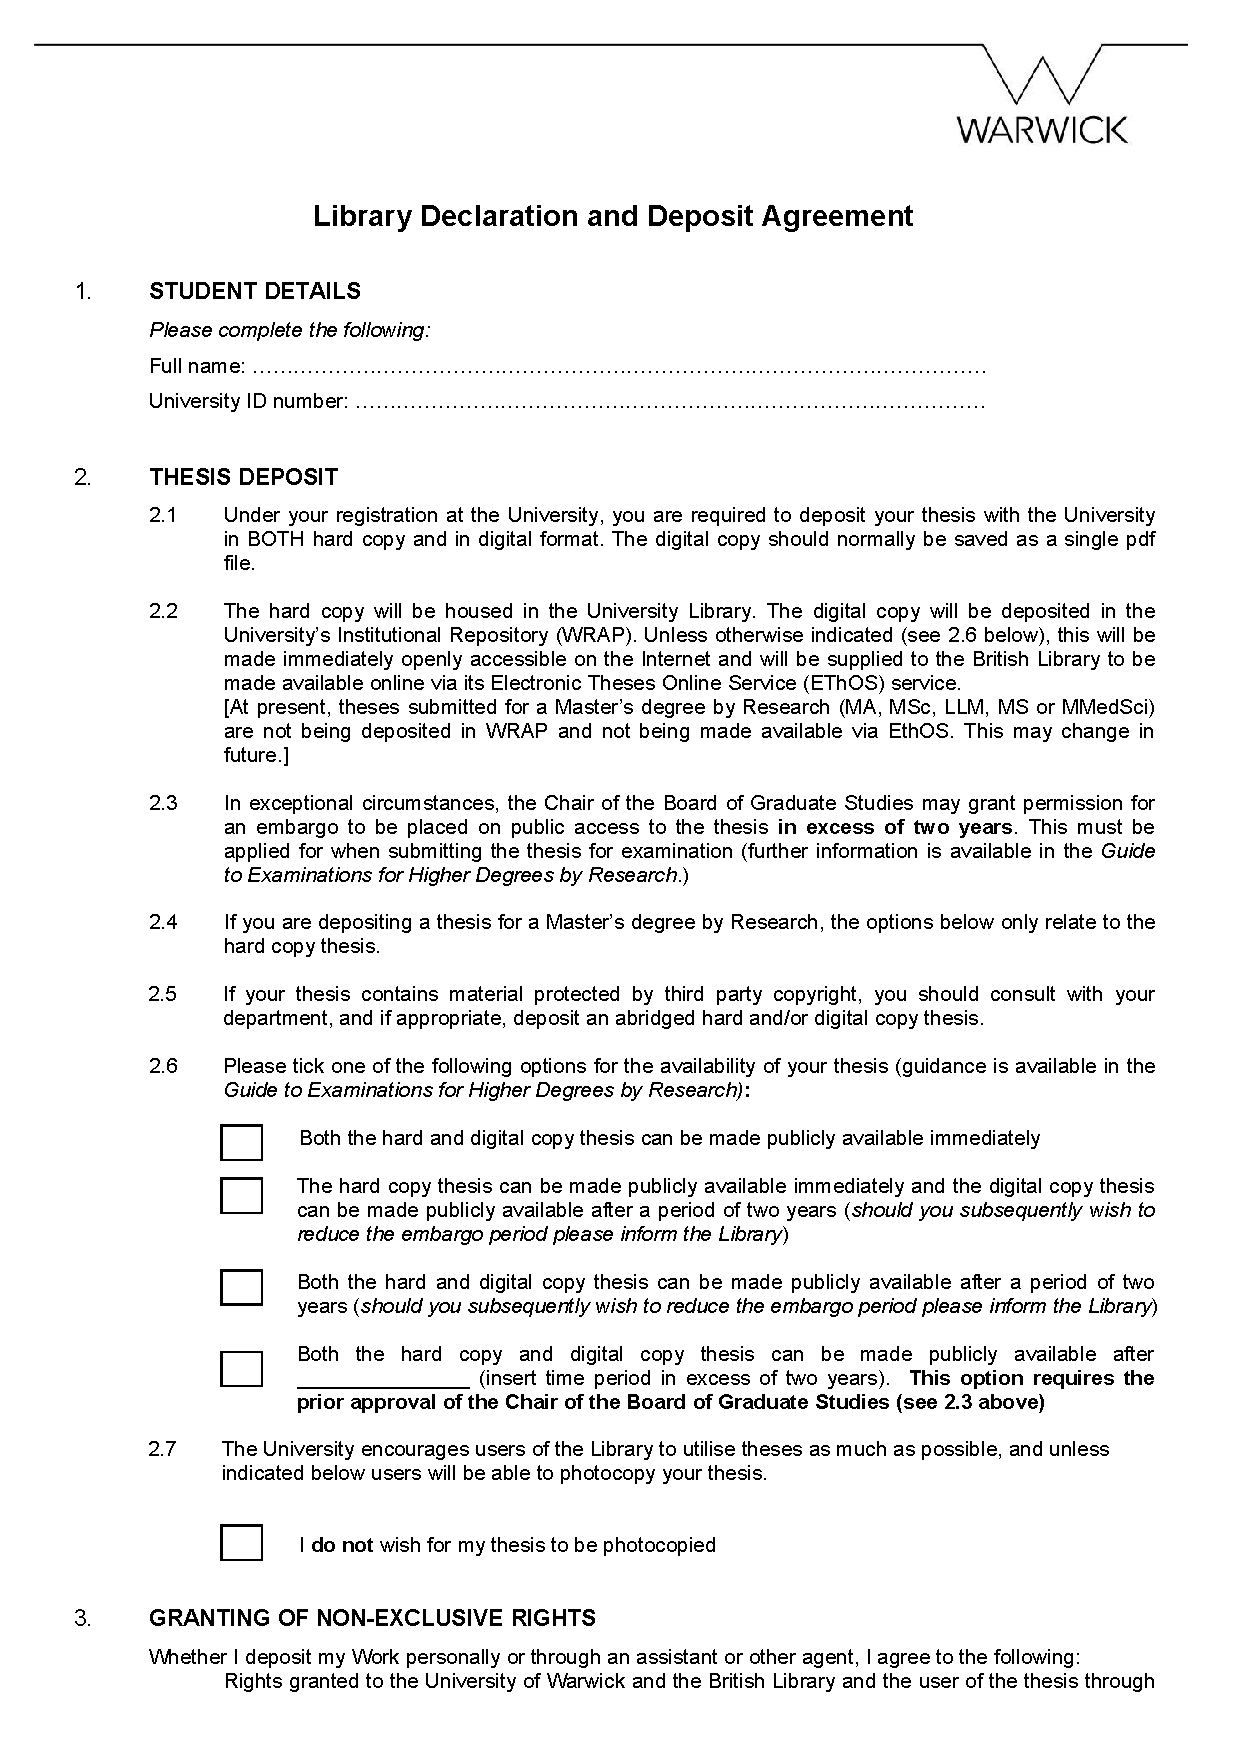
\includepdf[
	pages=-
]{Preamble/library_declaration_and_deposit_agreement.pdf}
\fi

\hypersetup{pageanchor=false}
\thesistitlebrandingpage
\hypersetup{pageanchor=true}

%%* Start roman page numbering here for contents, etc
%! Begins roman numerals start from page i.
\pagenumbering{roman}

\microtypesetup{protrusion=false} % disables protrusion locally in the document
\tableofcontents
\listoftables
\listoffigures
%{\let\clearpage\relax\listofalgorithms} % Uncomment if you have algorithms
\microtypesetup{protrusion=true} % enables protrusion


\include{Preamble/Acknowledgements}

% !TeX root = ../Thesis.tex

\begin{thesisdeclaration}

\noindent Parts of this thesis have been previously published by the author in the following:
\begin{itemize}
    \item lol i wish 1
\end{itemize}{}


\noindent Research was performed in collaboration during the development of this thesis, but does not form part of the thesis:
\begin{itemize}
    \item Titan 2018 paper
    \item LULI paper
    \item Filamentation papers
\end{itemize}{}

\end{thesisdeclaration}


% !TeX root = ../Thesis.tex

% Max 300 words, max 1 page

\begin{thesisabstract}
\begin{singlespace}

Abstract of max 300 words and max 1 page

Just did a bunch of stuff innit

\end{singlespace}
\end{thesisabstract}


%\include{Preamble/SponsorshipAndGrants}

% !TeX root = ../Thesis.tex

\glsaddall

% Having problems with extra blank page,
% problem is that the abstract ends with a newpage and this starts with a clearpage
% From: https://tex.stackexchange.com/questions/183097/renew-appendix-command-to-remove-blank-pages?rq=1
%\begingroup     
%\let\clearpage\relax

%\printnoidxglossary[type=\acronymtype,sort=word]

%\endgroup

% From: https://tex.stackexchange.com/questions/106987/custom-glossary-style-make-glossary-as-wide-as-textwidth
\newglossarystyle{tabx2col}{%
 % put the glossary in a longtable environment:
 \renewenvironment{theglossary}%
  {\begin{longtable}{L{0.07\textwidth}L{0.8\textwidth}}}%
  {\end{longtable}}%
 % Set the table's header:
 \renewcommand*{\glossaryheader}{}%
 % No heading between groups:
  \renewcommand*{\glsgroupheading}[1]{}%
 % Main (level 0) entries displayed in a row:
  \renewcommand*{\glossaryentryfield}[5]{%
    \glstarget{##1}{##2}% Name
    & ##3% Description
    \\% end of row
  }%
 % Sub entries treated the same as level 0 entries:
 %\renewcommand*{\glossarysubentryfield}[6]{%
  %\glossaryentryfield{##2}{##3}{##5}{##6}}%
 %% Nothing between groups:
 %\renewcommand*{\glsgroupskip}{}%
}

\printnoidxglossary[type=\acronymtype,sort=word,style=tabx2col]

%\printnoidxglossary[type=symbols,sort=def,style=tabx2col]

% Alternatively use this:
%\begin{thesisabbreviations}
%\end{thesisabbreviations}


%%* Start arabic numbering of main text here
\pagenumbering{arabic} %! Begins arabic numerals start from page 1.

% !TeX root = ../../Thesis.tex
\chapter{Introduction}
\label{chp:introduction}
The material presented in this thesis represents kinetic simulations of laser-plasma interactions (\acrshort{LPI}) relevant to direct-drive inertial confinement fusion (\acrshort{ICF}). In this introductory chapter, an overview of the goals of, and approaches to, inertial confinement fusion is given; including specific details of the `shock-ignition' (\acrshort{SI}) ICF scheme. We then review the previous work concerning laser-plasma interactions in direct-drive ICF, and motivate the use of kinetic modelling throughout this thesis. Finally, we offer an outline of the rest of the thesis.

\section{Inertial Confinement Fusion}
The basic concept of inertial confinement fusion (\acrshort{ICF}) is based on the Ulam-Teller design for a thermonuclear weapon (H-bomb), which uses radiation to compress thermonuclear fuel to the point where it undergoes nuclear fusion \citep{SpanishHistoryOfICF}.  Nuclear fusion is the process by which two light atomic nuclei overcome to electric repulsion between them and combine to form a new, heavier, nucleus and release energy proportional to the mass gap as kinetic energy of the fusion products. The reaction of choice in the thermonuclear weapon, and in most modern ICF designs, is deuterium-tritium (\acrshort{DT}) fusion. Equation \ref{eq:DTfusion} shows the \acrshort{DT}  reaction; first in the most commonly-presented formula, and then explicitly in terms of the ions and their neutron (superscript) and proton (subscript) numbers.

\begin{equation}\label{eq:DTfusion}
\begin{aligned}
	\text{D} + \text{T} &\longrightarrow \text{He}^4 + \text{n} + 17.6 \si{\mega\electronvolt}\\
	{}^2_1\text{H} + {}^3_1\text{H} &\longrightarrow {}^4_2\text{He} (3.5\si{\mega\electronvolt}) + {}^1_0\text{n} (14.1\si{\mega\electronvolt}).
\end{aligned}
\end{equation}
In order for a fusion reaction to be usable on earth, we require that it satisfies certain criteria: uses the lightest possible elements; reaction occurs at `reasonable' temperatures (on the order of $10 \si{\kilo\eV}$); reactants (fuel) are obtainable. Figure \ref{fig:crossSection} shows that the \acrshort{DT} reaction has the largest cross section / highest thermal reactivity of the several reactions which satisfy the above conditions.

\begin{figure}
 \centering
 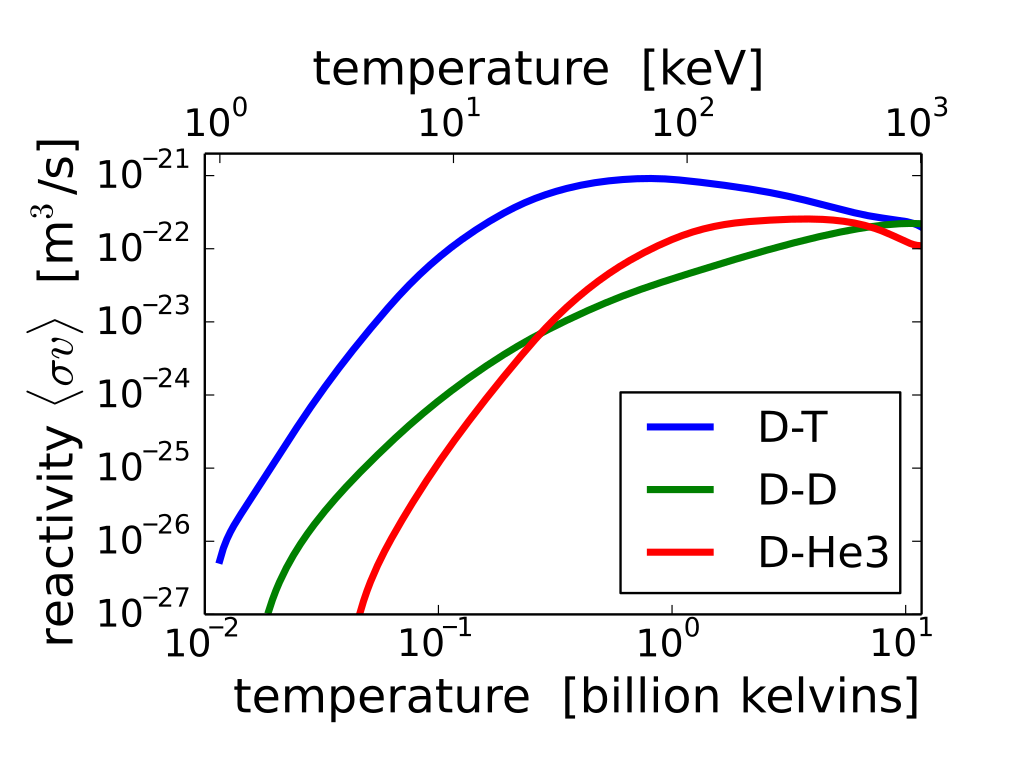
\includegraphics[width=0.7\columnwidth]{Chapters/C1_Introduction/crossSection.png}
 \caption{Thermal reactivity (product of interaction cross-section and velocity averaged over a Maxwellian) as a function of temperature: for deuterium-tritium, deuterium-deuterium (both interaction branches), and deuterium-helium nuclear reactions. Re-printed from \url{https://commons.wikimedia.org/wiki/File:Fusion_rxnrate.svg} under a Creative Commons 2.5 license, via Wikimedia Commons.} \label{fig:crossSection}
\end{figure}

In a thermonuclear weapon the radiation source is a fission bomb (also known as an `atom bomb' or `A-bomb'), which detonates and reaches very high temperatures, producing thermal x-rays which are channelled to compress the thermonuclear fuel. The fusion reaction which results from the high density and temperature conditions created in the compressed fuel is unconfined and, therefore, unsuited for energy generation. When lasers were proposed and realised, by \citet{Maser1958} and \citet{Maiman1960} respectively, scientists at Lawrence Livermore National Laboratory realised that lasers had the potential to ignite fusion explosions without using an atomic bomb. In 1972, \citet{Nuckolls1972} published a paper in Nature in which they used the LASNIX computer code to show that high-energy lasers could be used to compress hydrogen to super-high densities. Combined with small target pellets of fusion fuel, which will undergo burn before exploding (due to their inertia), the basic idea of inertial-confinement fusion (\acrshort{ICF}) was born. We now know that \acrshort{ICF} was demonstrated successfully in underground nuclear tests, just ten years after Nuckolls proposed it, but with a fission bomb as the driver, rather than a laser \citep{Evans2010}.




\subsection{Direct and indirect drive ICF}
Developments on the basic ICF scheme can be categorised by how the laser is used to perform the radiation compression of the fuel. In laser indirect-drive (\acrshort{LID}) models, fusion fuel is held inside a hollow chamber made of a high atomic number material. This structure is known as the hohlraum, from the German for `hollow space'. Lasers are then used to heat the inside walls of the hohlraum until they emit a bath of X-rays which heat the outer layer of the fuel capsule, causing the outer layer of the capsule to ablate and a rocket-effect-like implosion of the inner fuel. It is clear that this process is very similar to the indirect approach used to drive the thermonuclear explosion in the Ulam-Teller design. As such, the National Ignition Facility (\acrshort{NIF}) (US) and Laser M\'{e}gajoule (\acrshort{LMJ}) (France) are set-up for indirect-drive ICF, in order to support their respective country's nuclear weapons research programmes. An advantage of the indirect-drive technique is that the absorption and re-emission of laser energy by the hohlraum smooths the radiation which will drive the implosion.

Improvements in laser smoothing technology have made this advantage of \acrshort{LID} less obvious, and much research now focuses on laser direct-drive (\acrshort{LDD}). In laser direct-drive the laser beams are aimed at the target directly. Go through the steps: ablation; shocks; shocks; ignition. One limit to the success of any direct-drive scheme is the direct interaction of the laser with the coronal plasma. 





\subsection{Shock-ignition}
 This is a directly-driven central ignition scheme boosted by a strong shock.

\begin{figure}
 \centering
 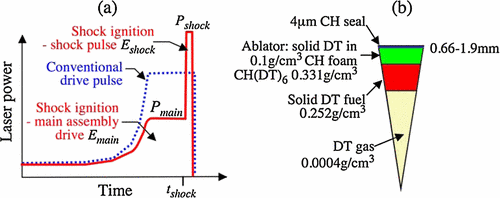
\includegraphics[width=0.9\columnwidth]{Chapters/C1_Introduction/SI_profile.png}
 \caption{\textbf{Reprinted with permission from \citet{Perkins2009}.} Shock-ignition design for the National Ingition Facility (NIF).} \label{fig:SI_laser}
\end{figure}


\section{Previous work}
\subsection{Laser-plasma interactions in shock-ignition}

Incident laser radiation drives a collective wave in a plasma to high amplitude, this wave then scatters in incident laser such that the beating of the laser and the scattered light ponderomotively drives electrons into bunches with a wavelength matching the initial plasma wave.

\subsection{Simulations}
\subsubsection{Kinetic models}
\subsubsection{Fluid models with kinetic effects}
Basically it's interesting that you can put some of these effects into a fluid model, such as here \citep{Tran2020}
\subsection{Experiments}

\subsection{Why PIC in this thesis?}
Question: doesn't PIC suck for predicting experimental observables? 

Need kinetics. Too expensive to use VFP for these laser-plasma interactions since the WFP velocity grid must be fine enough to resolve the electron quiver velocity. Also we have a PIC code in-house.

\section{Thesis Outline}
In the next five chapters, the wokr h uhuihuh uhi 

\begin{description}
	\item[Chapter 2] We present in Chapter \ref{chp:theory} the theory of laser-plasma interactions relevant to this thesis. We derive,... blah is introduced ... We describe the basic linear, quasi-linear, and non-linear theory required to understand normal modes; wave-particle interactions; and wave-wave instabilities, respectively, which are relevant to the coronal plasmas in direct-drive ICF.
	
	\item[Chapter 3] Here we present the EPOCH particle-in-cell (\acrshort{PIC}) code, which is used to perform all the simulations presented in this thesis, alongside a review of the PIC method for kinetic plasma simulations. Basic benchmarking of the code to the theory presented in Chapter \ref{chp:theory} is referenced, and we introduce several key diagnostics which are used throughout the thesis.
	 
	\item[Chapter 4] In this work, we use one-dimensional particle-in-cell 		
		simulations to show that there is a non-linear frequency shift caused  
		by kinetic effects, resulting in the growth of SRS in an inhomogeneous 
		plasma far exceeding the predictions of fluid theory, so-called 
		inflationary SRS or iSRS. We find that iSRS occurs over a wide range of 
		density scale-lengths relevant to shock-ignition and other directly-
		driven inertial confinement fusion schemes. Here we quantify the 
		intensity threshold for the onset of iSRS for shock-ignition relevant 
		parameters.
	
	\item[Chapter 5] In this chapter, results of one-dimensional PIC simulations are presented, which represent the first investigation into the practical possibility of using broadband to suppress inflationary SRS in shock-ignition. We show that for a decoupled broadband laser, the non-linear frequency shift must be taken into account when calculating the condition for suppression of iSRS. Next we consider the case of realistic shock-ignition schemes on three laser systems: frequency-tripled Nd : glass; Krypton Fluoride (KrF); and Argon Fluoride (ArF).
	\item[Chapter 6] In this chapter, we present work performed by the author while employed as a Junior Specialist at the University of California, San Diego between January and April 2020. We present modelling, performed by the author, of an experiment performed at the \acrlong{LULI} (France) by J. R. Marqu\`es \textit{et al.}. The experiment showed a small increase in SRS with an applied magnetic field, and this is recreated in our simulations. We then go on to investigate how the effect of the magnetic field depends on $\kld$ of the SRS electron plasma wave.
\end{description}

\section*{Conventions adopted in the thesis}
Unless otherwise stated in the text, all equations and physical quantities in this thesis are in SI units. Standard SI prefixes (k for kilo, T for tera- etc) are used. All numerically-calculated values are given to two significant figures, and written in scientific notation for values greater than 1000, and less than $1/1000$.

%\bibliographystyle{plainnat}
%\bibliography{Chapters/C1_Introduction/Introduction}


% !TeX root = ../../Thesis.tex
\chapter{Theory}
\label{chp:theory}

Remember to refer to Notes for Cours Ecole Doctorale, Advanced Theory of Plasmas, Ecole Polytechnique Fédérale de Lausanne (Saved on Mendeley)

\section{Pre-requisites}
This section assumes background knowledge of some commonly-taught UG and PG physics courses; including basic plasma physics concepts. A non-exclusive list is: Maxwell's equations; harmonic assumption and linearisation procedures

\section{Linear theory}
The aim of the linear theory of \acrshort{SBS} is to understand how the growth
 of the instability depends on factors such as: plasma density; laser intensity; and temperature.
\subsection{Dispersion curves and linear modes}
\subsection{Zoology/topology of modes}
\subsubsection{Beam acoustic modes}
\subsubsection{Electron acoustic modes}
ie on the omega,k diagram how many things are there that we should be worried
about? BGK modes, B\cite{Kruer96}
\subsection{Landau damping}

\section{Quasi-linear theory}
%\subsection{Landau damping}

A key aspect of quasilinear theory is its identification of the distinction between reso-
nant and non-resonant particles, scattering and diffusion \citep{Sagdeev2018}.

Bohm-Gross waves; Beam acoustic modes, other acoustic modes.
etc. Where are they and how do they relate? Ie the Bohm-Gross and Electron
Acoustic modes join at klD~0.53

\section{Nonlinear theory}
\subsection{Three-wave parametric instabilities}
\subsection{Nonlinear frequency shift}
\subsection{Nonlinear Landau damping}
%non-linear basis for trapping induced SRS modes found in \cite{Rose2001}, also
 %a thing called the nonlinear dielectric function

\subsection{Rosenbluth gain for SRS}

Since the instability we are concerned with is convective, we would like to understand what the maximum wave amplitude is for the daughter waves, according to the linear theory, in order to determine how SRS will grow in the fluid regime.

The derivation below follows the the steps laid out in \citet{Nishikawa1976}, with the following adapatations for this thesis:some steps written out in more explicit detail; notation changes, to improve the readability; and minor typographical corrections. 

We use our physical understanding of the system make the following assumptions:
\begin{enumerate}
	\item undamped EMW $\Gamma_1 = 0$
	\item strong damping and slow convection of EPW
	\item constant source at 0, maximum value at $+\infty$
	\item perfect matching at $x=0$, assume kappa is well-approximated by 
	$\kappa(x) = \kappa'(0)x$.
\end{enumerate}

Consider a three-wave parametric instability that takes place in a plasma slab with a density gradient in $x$ with a uniform pump. The density gradient leads to $x$-varying wavenumbers for the waves, so we define the `wavenumber mismatch' as $\kappa = k_0(x) - k_1(x) - k_2(x)$, where perfect matching is defined by the condition $\kappa(x=0) = 0$ and we insist that $\kappa = \kappa' x$. The daughter waves can be described by the following pair of partial differential equations:

\begin{equation}
 \left(\frac{\partial}{\partial t} + v_1\frac{\partial}{\partial x} + \Gamma_1 \right)a_1 = \gamma_0a_2\text{exp}\left(\frac{i\kappa'x^2}{2}\right)
\end{equation}

\begin{equation}
 \left(\frac{\partial}{\partial t} + v_2\frac{\partial}{\partial x} + \Gamma_2 \right)a_2 = \gamma_0a_1\text{exp}\left(\frac{-i\kappa'x^2}{2}\right);
\end{equation} 
where $\Gamma_{1,2}$ are the damping rates; $a_{1,2}$ the action amplitudes; and $v_{1,2}$ the group velocities of the two waves. 

WHAT ARE WE TRYING TO DO, WHAT MOTIVATES THIS TRANSFORM?

Recalling the definition of the Laplace transform of a function $f(t)$: $L\{f(t)\}= F(p) = \int_0^\infty e^{-pt} f(t) dt$ we take the Laplace transform of these equations to get






\section{Autoresonance}

\begin{figure}[ht]
    \centering
    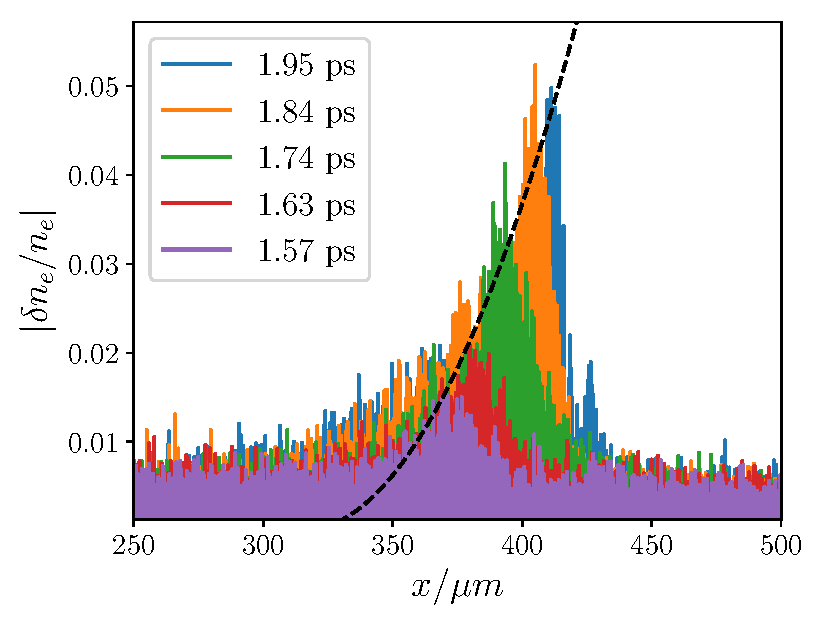
\includegraphics[width=0.8\columnwidth]{Chapters/C2_Theory/AR_diagnostic.pdf}
    \caption{Example of autoresonant growth in an EPOCH simulation with parameters: $n_{min} = 0.06 n_{\text{crit}}$; $n_{max} = 0.17 n_{\text{crit}}$; $T_e = 4.5\si{keV}$; $\text{nPPC}=10,000$; $I_0 = 2 \times 10^{15}\si{\watt / \centi\metre^2}$. Black dashed line comes from Chapman \textit{et al.} \citep{Chapman2012} formula.}
    \label{fig:AR_diagnostic}
\end{figure}{}

%\bibliographystyle{plainnat}
%\bibliography{Chapters/C2_Theory/Theory}


% !TeX root = ../../Thesis.tex
\chapter{Methods}
\label{chp:methods}

\section{The particle-in-cell method}
\subsection{Field solver}
\subsection{Interpolation to particles}
\subsection{Particle push}
\subsection{Interpolation to the grid}
\subsection{EPOCH}


\section{EPOCH benchmarking}
\subsection{Dispersion relations}
\subsection{Linear growth rates}

%\section{The coupled mode equation method}
%\subsection{The envelope equations}

%\section{LPSE benchmarking}
%\subsection{Linear growth rates}


\section{Diagnostics}
\subsection{Auto-resonance diagnostic}

% !TeX root = ../../Thesis.tex

\chapter{Inflationary stimulated Raman scattering in shock-ignition plasmas}
\label{chp:iSRS}
%\bibliographystyle{plainnat}
%\nobibliography{Bib/bib}

\title{Inflationary stimulated Raman scattering in shock-ignition plasmas}

This chapter is adapted, with the permission of AIP Publishing, from:
\begin{itemize}
  \item \bibentry{Spencer2020}.
\end{itemize}

In this chapter, results of one-dimensional (1D) particle-in-cell simulations are presented, which show that inflationary SRS (iSRS) can occur in shock-ignition plasmas and which characterise its threshold intensity in terms of the density scale length of the coronal plasma. Inflationary SRS refers to the enhancement of SRS above the levels predicted by fluid theory, caused by kinetic effects. The chapter begins with a review of the previous work on inflationary SRS in homogeneous plasmas, where the effect was first identified and understood. Then the case of iSRS in large-scale inhomogenous plasmas is considered, and a description in terms of autoresonance is presented. The code and initial conditions of the simulation are described, followed by a review of the signatures of iSRS and how they manifest in an inhomogeneous plasma. Finally the dependence of the inflationary SRS threshold intensity on density scale length for shock-ignition parameters, and the saturation of the instability are explored. The conclusion discusses the applicability of these results and ways to increase the experimental relevance of the simulations.


\section{Motivation and literature review}


\subsection{Homogeneous plasmas}
Inflationary SRS has been studied
extensively in the low-density homogeneous plasmas relevant to indirect-drive ICF on the NIF
\citep{Vu2002,Yin2006,Vu2007,Strozzi2007,Yin2008,Yin2012,Ellis2012}.
In attempting to explain experimental measurements of large SRS-reflectivities at high values of $k_\mathrm{EPW}\lambda_\mathrm{D}$
\citep{Fernandez2000,Montgomery2002}, it was suggested that some mechanism caused a reduction in the Landau damping
rate by four to five times, compared to the damping for a Maxwellian plasma \citep{Montgomery2002}.
Anomalously large SRS-reflectivities were recreated in simulations \citep{Vu2001,Vu2002}, and were explained by
reference to O'Neil's 1965 model of reduced EPW  damping caused by electron-trapping \citep{ONeil1965}.
In homogeneous plasmas, iSRS occurs when an SRS EPW grows to a point where it can trap electrons for one
complete bounce period or longer, without them becoming de-trapped due to velocity-space diffusion or
side-loss \citep{Vu2002}. This trapped electron population leads to modification of the distribution
function, in the form of a locally flattened region around the EPW phase velocity.
This translates to a modification of the dielectric properties of the plasma, resulting in a reduction in
the EPW's associated Landau damping rate \citep{ONeil1965,Vu2002}, and increased SRS growth.

 Key results of previous studies of inflationary SRS in homogeneous plasmas include: a theory for the saturation
 of iSRS in terms of EPW bowing and the trapped-particle modulation instability \citep{Yin2008}; the derivation
 of an inflation threshold intensity in terms of competition between trapping in the EPW and diffusion in
 velocity space \citep{Vu2007}; and the description of iSRS in terms of a transition from convective to absolute
 growth \citep{Wang2018}. Inflationary SRS has also been identified as an important mechanism in simulations  with ensembles of laser speckles \citep{Yin2012,Winjum2019}.

\subsection{Inhomogeneous plasmas}

 In the large-scale inhomogeneous plasmas associated with shock-ignition ($L_n \simeq 300-1000 \si{\micro\metre}$) the mechanism and effects of inflationary SRS have received much less attention. The few papers which do refer to iSRS in SI inhomogeneous plasmas assume that the explanation of iSRS in a homogeneous plasma in terms of reduced Landau damping also applies to iSRS in an inhomogeneous plasma. However, iSRS in an inhomogeneous plasma actually happens by a different mechanism. In the case of a homogeneous plasma, reduced Landau damping due to electron-trapping in the EPW leads to an increase of the SRS growth rate which, if sufficiently large, can cause a transition from convective to absolute growth \citep{Wang2018}. For an inhomogeneous plasma, where the growth of SRS is always convective, the reduction in Landau damping associated with trapping in the EPW has no net effect on the convective gain \citep{Williams1991}.
 
 While the local SRS growth rate may depend on the EPW damping rate in an inhomogeneous plasma, the region of SRS convective growth is also extended, leading to a net Rosenbluth gain \citep{Rosenbluth1972} which is independent of Landau damping \citep{Williams1991,Liu1994}. We therefore look to another non-linear effect caused by the trapped electrons in the SRS EPW, the non-linear frequency shift \citep{Morales1972}. In an inhomogeneous plasma, the frequency shift resulting from electron-trapping can compensate for the wave-number mismatch on propagating up the density gradient, thereby allowing
 growth over a larger region - an auto-resonance \citep{Chapman2010,Chapman2012}. \citet{Chapman2012} proposed this theory for iSRS in an inhomogeneous $(L_n \lesssim 100
 \si{\micro\metre})$ plasma close to the hohlraum wall in indirect-drive ICF. They demonstrated the auto-resonant
 interaction \cite{Chapman2010} between the non-linear frequency shift associated with electron-trapping in EPW
 and the wave-number mismatch caused by plasma inhomogeneity; which allows larger SRS gain \cite{Chapman2012}.


 Inflationary SRS has been suggested as the cause of SRS from low densities
 in simulations of LPI in shock ignition \citep{Klimo2014}. Sub-scale shock-ignition experiments have detected
 SRS scattered light from densities $0.09 - 0.16 n_\mathrm{cr}$, where the inflationary mechanism should be important \citep{Cristoforetti2017}. Recent full-scale ($L_n > 500
 \si{\micro\metre}$, $T_e = 5\si{\kilo \electronvolt}$) directly-driven experiments have detected significant SRS-reflected light from densities $0.15 - 0.21 n_{\mathrm{cr}}$ \citep{Rosenberg2020}. Another full-scale ($L_n = 450
 \si{\micro\metre}$, $T_e = 4.5\si{\kilo \electronvolt}$) SI experiment measured SRS-reflected light from densities between $0.05 - 0.15 n_{\mathrm{cr}}$. Under the conditions of the experiment, $k_{\mathrm{EPW}}\lambda_D$ ranges from $0.3 - 0.6$ and the measured SRS is assumed to be inflationary in origin \citep{Baton2020}.
 For a single laser speckle in an inhomogeneous plasma with density
 scale-length $L_n\simeq 70 \si{\micro\metre}$, \citet{Riconda2011} demonstrated
 that iSRS  was associated
 with electron-trapping in the EPW. By varying $a_0=eE_0/c m_e \omega_0$ from 0.03 to 0.06, i.e. an increase in
 laser intensity from $1.0\times10^{16} \si{W/\centi\metre^2}$ to $4\times10^{16} \si{W/\centi\metre^2}$, they showed
 a transition to iSRS.

\section{Code and initial conditions}\label{sec:code&IC}


As described in Chapter \ref{chp:methods}, all simulations are performed using the EPOCH \citep{Arber2015} particle-in-cell code. The simulation parameters are chosen to achieve our primary aim of identifying plasma parameters where iSRS may occur; which does not require large simulations of the entire LPI system. The simulations all used a domain size of $L_x = 100\si{\micro\metre} $ and ran to $T_\mathrm{end} = 2\si{\pico\second}$
with 2048
particles per cell (PPC) for the electron species.
We treat the ions as a neutralising background population, since we simulate only a two pico-second interval of SRS
development, during which ion dynamics will not become important \citep{Rousseaux2006}.
For the plasma parameters laid out above, electron-ion collisions occur on a characteristic timescale of approximately
$7 \si{\pico\second}$ at the highest density probed, $0.22n_\mathrm{cr}$. Since the inflationary Raman process we
are investigating takes place
on a sub-picosecond timescale, we do not include collisions in our simulations.
The plasma density profiles are given by the expression $n(x) = n_\mathrm{min}\mathrm{exp}(x/L_n)$ and can be seen in Table
\ref{tab:densities}.

\begin{table}[ht]
    %\begin{ruledtabular}
    \begin{center}
    \begin{tabular}{|c|c|c|c|}
    \hline 
    $L_n/\si{\micro \metre}$  & $n_\mathrm{mid}/n_\mathrm{cr}$ & $(n_\mathrm{min},n_\mathrm{max})/n_\mathrm{cr}$ &$(k\lambda_\mathrm{D_{min}},k\lambda_\mathrm{D_{max}})$\\
    \hline \hline
    300& 0.15  & $(0.13,0.18)$ & $(0.28,0.37)$\\
    500 & 0.12 &$(0.11,0.13)$ & $(0.37,0.41)$\\
    500 & 0.15 & $(0.14,0.17)$& $(0.29,0.35)$ \\
    500 & 0.20 & $(0.18,0.22)$& $(0.21,0.27)$\\
    1000 & 0.15 & $(0.14,0.16)$ & $(0.31,0.32)$ \\
    \hline
    \end{tabular}
    \end{center}
    %\end{ruledtabular}
        \caption{\label{tab:densities}
        Summary of density profiles and $k_{EPW}\lambda_\mathrm{D}$ values in each simulation. $L_n=n_e/(dn_e/dx)$ evaluated at $n_\mathrm{mid}$. For all but the case centred at $0.2n_\mathrm{cr}$, $k_\mathrm{EPW}\lambda_\mathrm{D} > 0.28$ and we are in the strongly kinetic regime. The total range of $k_\mathrm{EPW}\lambda_\mathrm{D}$ probed is 0.21-0.41.
        }
\end{table}


We simulate a frequency-tripled Nd:glass laser with vacuum wavelength $\lambda_0 = 351\si{\nano\metre}$, polarised in the $y$-direction. The laser intensity was varied in 20 logarithmically evenly-spaced increments between $10^{14}$\si{W/\centi\metre^2} and $10^{16}$\si{W/\centi\metre^2}, with a half-Gaussian temporal profile followed by a flat top, and a rise-time of 50 laser periods.
We use absorbing boundaries for the fields and thermal for the particles; these replace any particle leaving the
simulation with an incoming particle with velocity consistent with a Maxwellian plasma based on the initial temperature of $4.5$\si{keV}.


EPOCH uses a pseudorandom number generator (PRNG) to generate the initial particle distribution.
Each simulation was repeated 10 times with a different PRNG seed, allowing us to determine the sensitivity of
SRS to plasma fluctuations.
This allowed us to calculate both the mean and standard deviation of the intensity of the light scattered through SRS.

\begin{figure}[ht]
 \centering
 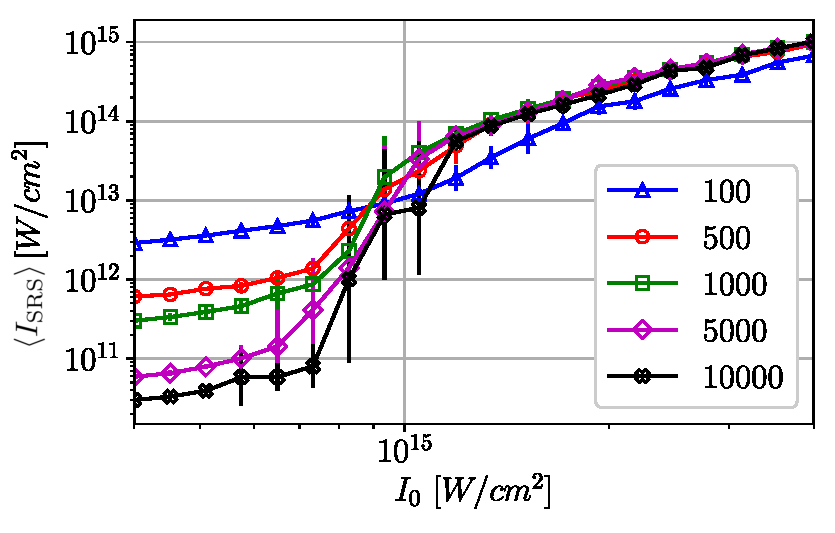
\includegraphics[width=0.8\columnwidth]{Chapters/C4_iSRS/fig1.pdf}
 \caption{Time-averaged intensity of SRS scattered light for a homogeneous simulation ($n_e=0.15n_\mathrm{cr}$, $T_e = 4.5$\si{\kilo \electronvolt}) with different numbers of particles
 per cell. Relative errors are given by one standard deviation of the SRS scattered light intensity as calculated from ten simulations.} \label{fig:convergence}
\end{figure}

SRS amplifies fluctuations in the plasma, and so is sensitive to number of particles per cell used in the simulation, as can be seen in Figure \ref{fig:convergence}.
In this figure, the intensity of SRS back-scattered light (denoted in this paper by $\langle I_{\mathrm{SRS}}\rangle$) is plotted against the incoming laser intensity $I_0$ ranging between
$0.4 - 4.0 \times 10^{15}$\si{W/\centi\metre^2} for a homogeneous plasma with $n_e=0.15n_\mathrm{cr}, T_e = 4.5$\si{\kilo \electronvolt}, for different numbers of
particles per cell.
At low incident intensity, $\langle I_{\mathrm{SRS}}\rangle$ is inversely proportional to the number of PPC used. This is as we
would expect for the case of simple convective amplification \citep{Rosenbluth1972} of the product of two quantities ($E_y,B_z$) which vary as background PIC noise, which is proportional to $1/\sqrt{\mathrm{PPC}}$.
The upper saturated level of  $\langle I_{\mathrm{SRS}}\rangle$ is robust to the number of PPC for $\mathrm{PPC} > 100$.
The transition between these two levels represents the change from standard convective amplification of SRS to enhanced
growth of SRS due to trapping (inflationary SRS), hence we call this the inflation threshold.
The existence of an inflation threshold is also robust to the number of particles per cell for $\mathrm{PPC} > 100$.

In the region containing the inflation threshold, the error associated with the intensity of SRS scattered light is largest. This suggests that inflationary SRS is very sensitive to the initial distribution of particles in the simulation domain, and that a statistical analysis of the mean and standard deviation of intensity across different random seeds will be important if we are to determine the iSRS threshold intensity accurately.


\section{Diagnosing iSRS in inhomogeneous plasmas}\label{sec:signatures}
Three signatures of inflationary SRS observed in the literature for homogeneous plasmas are: a threshold intensity past which scattering of laser light is enhanced above the level predicted by fluid theory \citep{Vu2007}; electron-trapping in the SRS EPWs leading to local flattening of the distribution function at the EPW phase velocity \citep{Vu2002}; and the growth of down-shifted SRS EPWs and a continuum of beam-acoustic modes (BAMs) \citep{Yin2006}.
In what follows we show that all of these signatures are also present for iSRS in an inhomogeneous plasma, despite the instability arising through an auto-resonance rather than a transition from convective to absolute growth.

\subsection{Inflation threshold}
We consider first the existence of  a threshold intensity past which SRS growth is enhanced, by several
orders of magnitude, above the predictions of fluid theory; this has been seen in experiments \citep{Kline2006} and simulations \citep{Vu2002,Yin2006,Vu2007,Riconda2011}.

In order to identify kinetic inflation of the SRS scattered light intensity in our PIC simulations,
we use the simple fluid model presented in Section \ref{diag:threshold} to calculate and compare the intensity of SRS scattered light in the absence of kinetic effects.

The red circular markers in Figure \ref{fig:kineticVsfluid} show the results of applying this method to the case of a $500\si{\micro\metre} $ density scale-length plasma, with the density profile centred at $0.15n_\mathrm{cr}$, for incident laser intensities ranging from $10^{14} - 10^{16}$\si{W/\centi\metre^2}. The blue triangular markers show the intensity of SRS scattered light calculated from the equivalent kinetic EPOCH simulations. The relationship between the kinetic and fluid results changes as the incident laser intensity increases. At low intensities the fluid and kinetic models are well matched, but not identical, suggesting that there is always some kinetic element to the SRS behaviour in these simulations.

Continuing this analysis to intensities $<10^{13}$\si{W/\centi\metre^2} (well below those relevant to shock-ignition) shows that the two methods converge for low intensities, where the behaviour is purely fluid. Once the incident laser intensity exceeds  $I_\mathrm{threshold} \sim 1.4\times10^{15}$\si{W/\centi\metre^2}, the intensity of SRS scattered light measured in the kinetic simulations exceeds the fluid prediction by between one and three orders of magnitude, until the intensity reaches $I_0 = 10^{16}$\si{W/\centi\metre^2}, where it appears to saturate. In the fluid model, $\langle I_{\mathrm{SRS}}\rangle$ is a smooth function of incident laser intensity and we cannot define such a threshold intensity. This implies that kinetic effects in our simulations are responsible for the increase in $\langle I_{\mathrm{SRS}} \rangle$ and that we have observed iSRS. The fluid estimate shows no sign of saturating at high intensities, since the Rosenbluth gain formula used is based on unbounded linear SRS growth over the resonance region $\ell$ and the model does not include pump depletion.

By constructing plots such as these, which show the fully kinetic PIC results alongside results from our simple fluid model, we are able to identify the iSRS threshold as the point past which the kinetic and fluid models differ by at least one order of magnitude.


\begin{figure}[ht]
    \centering
    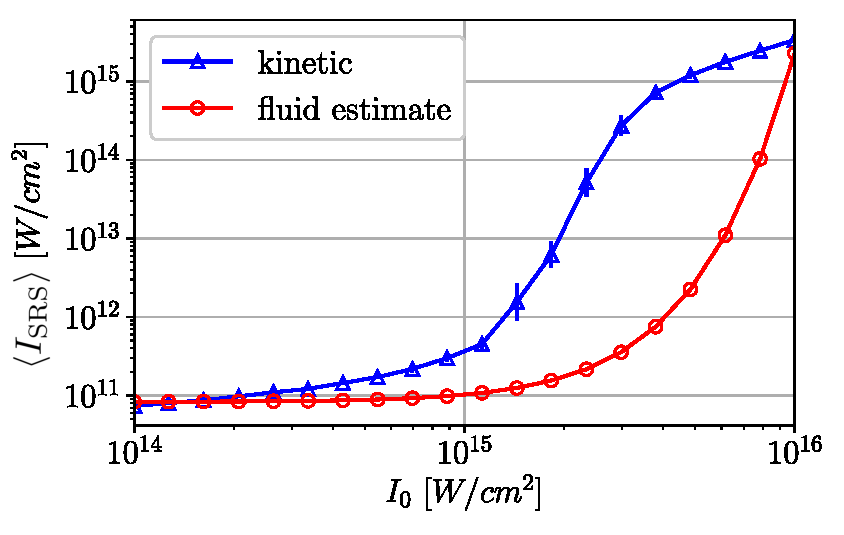
\includegraphics[width=0.8\columnwidth]{Chapters/C4_iSRS/fig2.pdf}
    \caption{
        Blue triangular markers show the intensity of SRS scattered light calculated using the fully-kinetic EPOCH code for parameters: $L_n = 500 \si{\micro\metre} $ and $n_{\mathrm{mid}} = 0.15n_\mathrm{cr}$.
        Red circular markers show the intensity of SRS scattered light calculated, for the same plasma parameters, from the fluid model presented above.
        The initial noise level in the fluid model was calculated from a PIC simulation without the laser driver: $I_\mathrm{noise}=\langle E_yB_z\rangle_{x,t} / \mu_0 = 8\times 10^{10} \si{W/\centi\metre^2}$.}
    \label{fig:kineticVsfluid}
\end{figure}{}

\subsection{Electron trapping}


\begin{figure}[!ht]
 \centering
 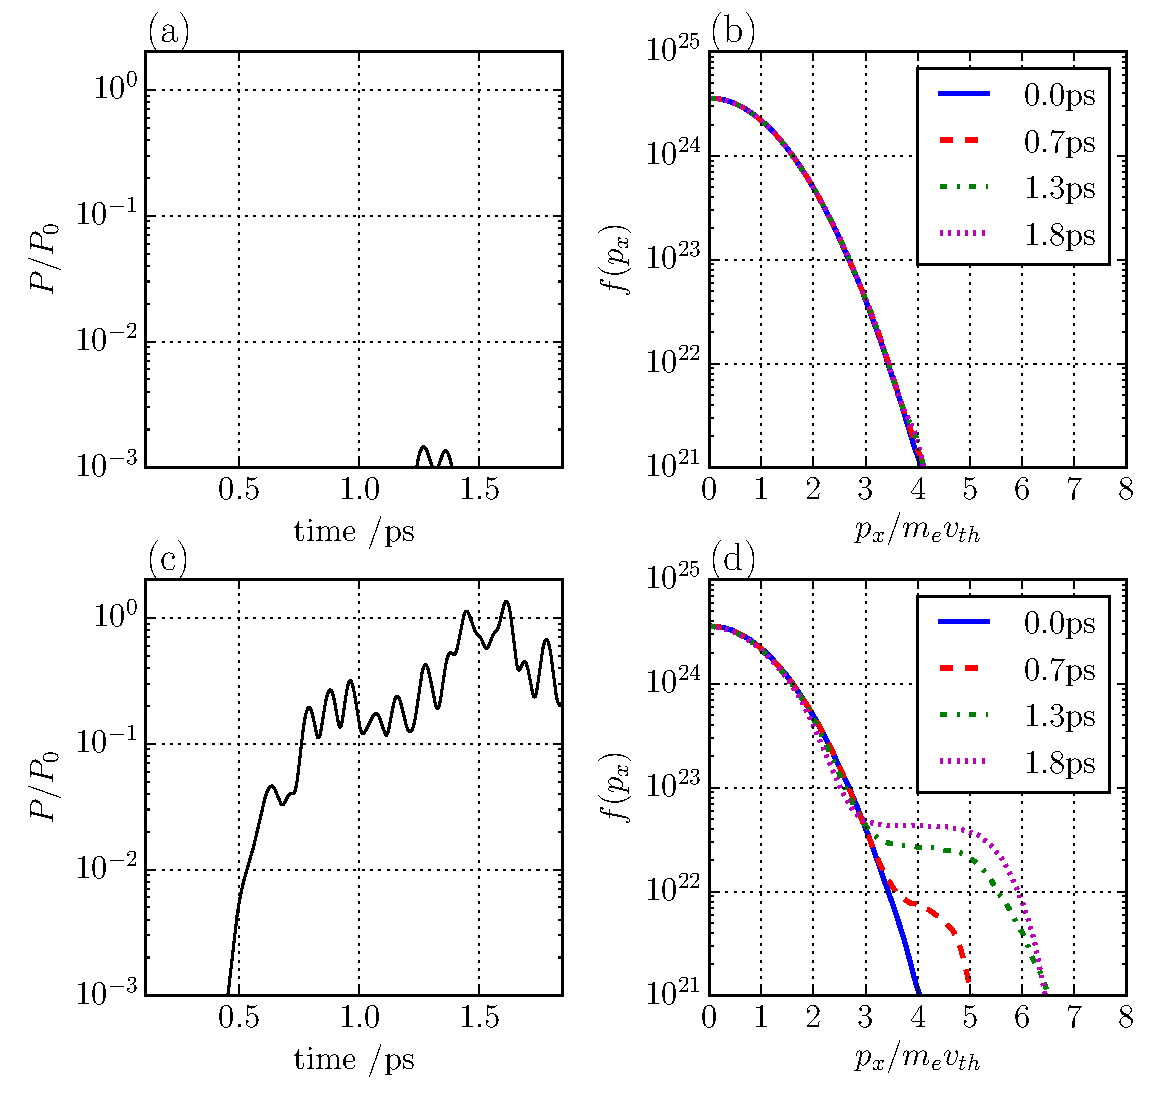
\includegraphics[width=0.8\columnwidth]{Chapters/C4_iSRS/fig3_3a_3b_3c_3d.pdf}
 \caption{Time-resolved comparison of SRS-reflectivity (a,c) and electron distribution 
 functions (b,d) for two simulations with parameters: $L_n = 500 \si{\micro\metre} $; centred
 at $0.15n_\mathrm{cr}$; and $T_e = 4.5$\si{\kilo\electronvolt}. The distribution function of
 electron momentum is averaged over the entire spatial domain at four times, normalised to the initial thermal momentum. Panels (a,b) have an incident laser intensity below the threshold for inflationary SRS; $I_0 = 1.13\times10^{15}$\si{W/\centi\metre^2}. Panels (c,d) have an incident laser intensity above the iSRS threshold; $I_0 = 4.83\times10^{15}$\si{W/\centi\metre^2}.}
 \label{fig:reflAndDist}
\end{figure}

A second signature of iSRS, as reported in the literature for homogeneous plasmas, is electron-trapping in the SRS electron plasma waves, leading to a
non-linear frequency shift and enhanced SRS-reflectivies at large $k\lambda_\mathrm{D}$ \citep{Vu2002}.
A typical manifestation of this, for our inhomogeneous simulations, is shown in Figure \ref{fig:reflAndDist}. Figure \ref{fig:reflAndDist}
shows the instantaneous SRS-reflectivity measured at the left boundary of the simulation domain (a,c), alongside the box-averaged electron
distribution function at four times (b,d), for two simulations with laser intensities above and below the iSRS threshold.
Sub-figures \ref{fig:reflAndDist} (a,b) show that, when driven below threshold, the distribution of electron momenta is Maxwellian throughout the simulation, and that the maximum instantaneous power in SRS-refle\
cted light is consequently very low ($P \sim 10^{-3}P_0$). In sub-figures (c,d), where the incident laser intensity is well above the iSRS threshold, we see that the power in SRS-reflected light is correlated wi\
th the growth of a non-Maxwellian tail in the distribution function, corresponding to an electron population trapped in the SRS electron plasma waves.
There is a general trend of increasing SRS-reflected light that correlates with
the increasing trapped electron population.


\subsection{Nonlinear frequency shift}
Electron-trapping in the SRS-driven EPW causes a time-dependent non-linear frequency shift of
the EPWs \citep{Morales1972,Kline2006}, and the growth of a sequence of beam-acoustic modes \citep{Yin2006}; this is the third signature of iSRS.

\begin{figure}[h!]
    \centering
    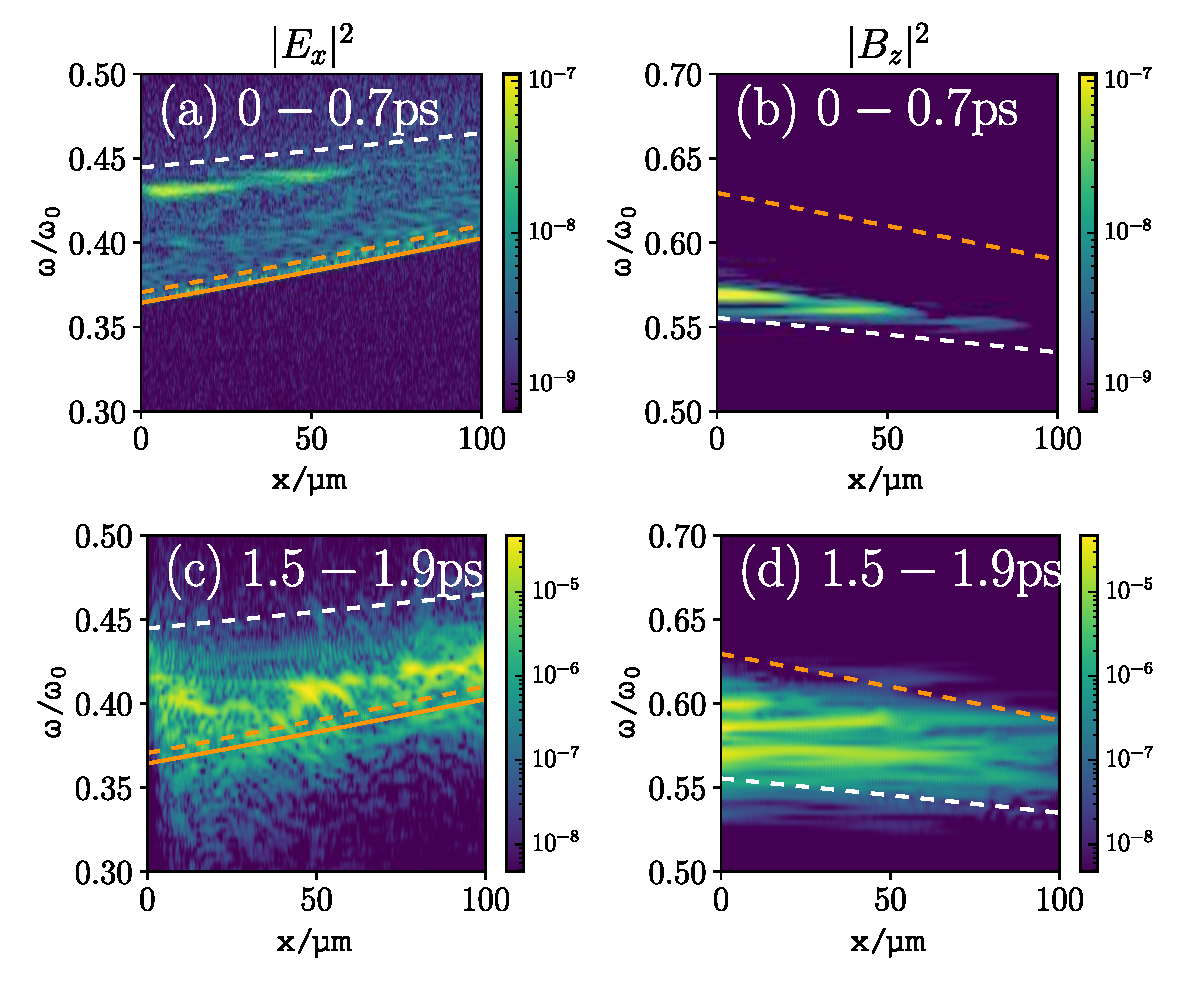
\includegraphics[width=0.8\columnwidth]{Chapters/C4_iSRS/fig4_4a_4b_4c_4d.pdf}
    \caption{Top panels show the spectra of electrostatic (a) and electromagnetic (b) waves over the period $0-0.7\si{\pico\second}$.
    The white (orange) dashed lines represent the linear predictions for the spectra of backward (forward) SRS. The bottom panels show the same spectra calculated over the period $1.5-1.9\si{\pico\second}$. The \
$E_x$ ($B_z$)
    spectrum is significantly down-shifted (up-shifted), demonstrating a trapped population of electrons in the EPW \citep{Yin2006}.
    The orange solid line represents the plasma frequency $\omega_{\mathrm{pe}}$ for the simulation parameters: $L_n = 500 \si{\micro\metre} $ centred at $0.15n_\mathrm{cr}$ and $I_0 = 4.83\times10^{15}$\si{W/\centi\metre^2}.}
    \label{fig:downshift}
\end{figure}{}

Figure \ref{fig:downshift} shows the spatially resolved frequency spectra of
EPWs (a,c) and EMWs (b,d) at 0-0.7ps
(a,b) and 1.5-1.9ps (c,d). In panels (a,b), the signal maxima sit very close to
the white dashed line, which represents the frequencies predicted by the SRS
matching-conditions for the original Maxwellian plasma. This means that, at
early time, the SRS EPWs and their associated back-scattered light
waves are excited at the frequencies matching those of the linear theory
without trapping.
They are slightly down-shifted from the analytical prediction, which suggests
that the trapping
becomes important almost immediately in our simulations.
At later time, Figure \ref{fig:downshift} (c) shows that the EPW spectrum is
down-shifted in frequency
at every location in the simulation domain, including to frequencies below the
plasma frequency for the original Maxwellian plasma (orange solid line).
This is evidence of a large trapped particle population removing energy from
the wave, causing the frequency of the wave
to decrease such that energy is conserved \citep{Morales1972}. We also note that
in Figure \ref{fig:downshift} (d) the back-scattered light spectrum is
up-shifted in frequency space, so as to maintain frequency matching. As well as obvious up-shift of the electromagnetic spectrum, we can also see more general broadening as we move from Figure \ref{fig:downshift} (b) to (d). This could be caused by waves from a higher density propagating to smaller $x$, so that at a particular location the spectrum covers waves from a range of densities.



\subsection{Beam acoustic modes}
\begin{figure}[ht]
    \centering
    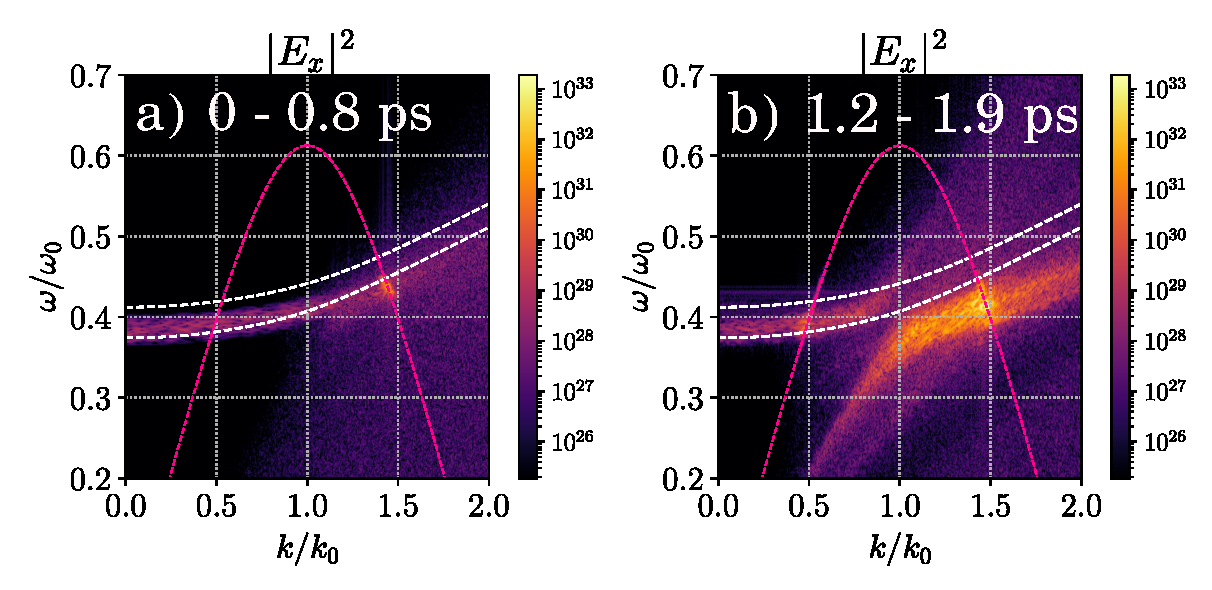
\includegraphics[width=0.8\columnwidth]{Chapters/C4_iSRS/fig5_5a_5b.pdf}
    \caption{(a) 2D FFT of $E_x$ over the period $ 0 - 0.8 \si{\pico\second}$. (b) 2D FFT of $E_x$ over the period $1.2 - 1.9                                                                              
    \si{\pico\second}$.
    The white dashed lines represent the analytical dispersion relations corresponding to the minimum (bottom line) and maximum (top line) plasma densities,
    assuming a Maxwellian electron distribution.
    The pink dashed line shows the Stokes line for down-shifted EM waves.
    Simulation parameters: $L_n = 500 \si{\micro\metre} $ centred at $0.15n_\mathrm{cr}$
    and $I_0 = 4.83\times10^{15} \si{W/\centi\metre^2}$.
    }
    \label{fig:BAM}
\end{figure}{}

Further evidence for a large trapped particle population can be seen in the growth of a beam acoustic mode in the electrostatic $(\omega,k)$ spectrum. Figure \ref{fig:BAM} shows the electrostatic dispersion relation from a simulation; it is calculated by taking a 2D Fourier transform of the $E_x$ field over the entire spatial domain, and over two distinct time intervals. At early time, shown in Figure \ref{fig:BAM} (a), electron plasma waves are excited, from background noise, between the two white dashed curves. These
represent the Bohm-Gross dispersion relations $\omega_\mathrm{EPW}^2 = \omega_{\mathrm{pe}}^2 + 3v_\mathrm{th}^2k_\mathrm{EPW}^2$ for the highest density in the
domain (top line) and the lowest density (bottom line). According to fluid theory, SRS will grow where the  Stokes branch, defined by $(\omega-\omega_0)^2 = \omega_{\mathrm{pe}}^2 + c^2(k-k_0)^2$, intersects
with this dispersion curve. This fluid-SRS signal can be seen in Figure \ref{fig:BAM} (a).

The right hand panel of Figure \ref{fig:BAM} shows the EPW dispersion relation calculated from the simulation between $1.2 - 1.9
\si{\pico\second}$. Inspection of the distribution function in Figure \ref{fig:reflAndDist} shows that, at these times, the distribution
function is modified from the initial Maxwellian and has a large flattened region, which acts as an effective beam population
\citep{Yin2006}. According to  linear theory, this change in the distribution function $f$ changes the kinetic dispersion relation for the electrostatic waves in the system, defined by: $\epsilon(\omega,k) = 1 - \frac{q_e^2}{\epsilon_0m_ek}\int\frac{\partial{f}/\partial{v}}{v-\omega/k} dv = 0$.
This change in the dielectric properties of the plasma is realised in the $(\omega,k)$ spectrum as a continuum of beam acoustic
modes \citep{Yin2006}, this is the large spectral feature in the right hand panel of Figure \ref{fig:BAM} that sits strictly below
the Bohm-Gross dispersion curves.
These beam acoustic modes are frequency downshifted, recovering the result from Morales and O'Neil's non-linear analysis\citep{Morales1972}. The maximum of the BAM signal at $k \sim 1.5k_0$ is the intersection of the BAM with the Stokes
branch, the new location of SRS growth.

We can also see in Figure \ref{fig:BAM} (b) a signal at $k\sim 0.5k_0$ which sits on the intersection of the Stokes branch with the range of EPWs satisfying the Bohm-Gross dispersion relations. This represents forward-scattered SRS EPWs, which have not undergone a significant frequency shift. For all the simulations presented in this paper, when driven above threshold, the power in forward SRS scattered light is of the order $P \sim 10^{-3} P_0$ or lower, and is therefore energetically unimportant.


\section{Intensity threshold and hot electron scaling}\label{sec:paramScan}
Using the method developed in Section \ref{sec:signatures} for locating the inflation threshold, and the analysis of electron trapping and downshifted EPWs to ensure that the SRS observed is inflationary in origin, we investigate how iSRS depends on various plasma parameters relevant to shock-ignition. Using the PIC simulation set-up as in Section \ref{sec:code&IC} (with the same simulation domains, plasma densities, and temperatures), we varied the plasma density scale-length across the range
of values predicted for shock-ignition $(300\si{\micro\metre} - 1000\si{\micro\metre})$ \citep{Ribeyre2009}. As well as varying the density scale-length, we also centred the density profiles at different values of density. Figure \ref{fig:paramScan} shows the result of this parameter scan.

\begin{figure}[!ht]
     \centering
    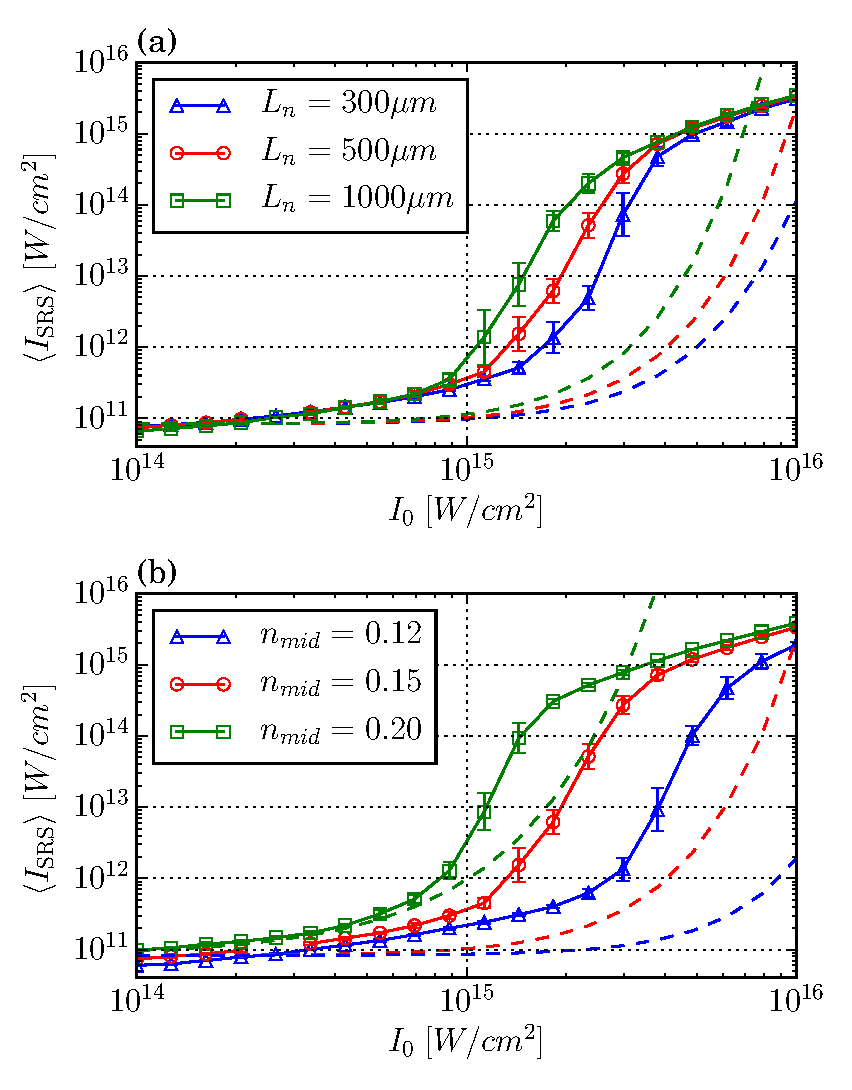
\includegraphics[width=0.7\columnwidth]{Chapters/C4_iSRS/fig6_6a_6b.pdf}
    \caption{
    (a)  Relationship between incident laser intensity and the intensity of SRS scattered light for three different density scale-lengths, with plasma density profiles centred at $0.15n_\mathrm{cr}$.
    (b) Relationship between incident laser intensity and the intensity of SRS scattered light for three simulations with $L_n=500\si{\micro\metre}$ centred at three different densities.
    Each coloured dashed line represents the prediction of the fluid model presented in Section \ref{sec:signatures} for the same parameters as the solid line of the same colour.
    }
    \label{fig:paramScan}
\end{figure}

\begin{figure}[ht]
   \centering
    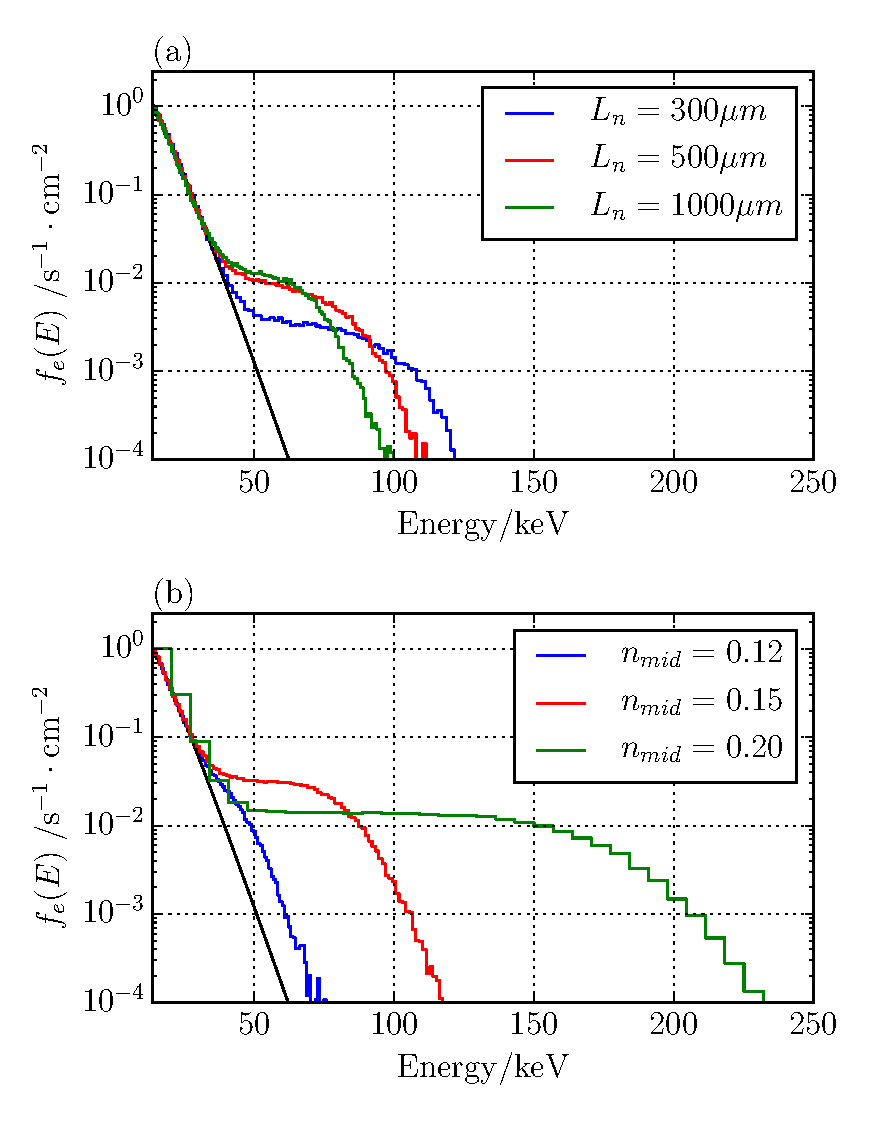
\includegraphics[width=0.7\columnwidth]{Chapters/C4_iSRS/fig7_7a_7b.pdf}
    \caption{(a) Hot electron flux through the right boundary in three simulations with parameters: $I_0 = 2.98\times 10^{15} \si{W / \centi \metre^2}$; $n_\mathrm{mid}=0.15 n_\mathrm{cr}$; $L_n=300,500\
,1000\si{\micro\metre}$.   (b) Hot electron flux through the right boundary in three simulations with parameters:
   $I_0 = 6.16\times 10^{15} \si{W / \centi \metre^2}$;  $L_n=500\si{\micro\metre}$; $n_\mathrm{mid}=0.12,0.15,0.20 n_\mathrm{cr}$ respectively. Each distribution is normalised to its maximum value. The smooth b\
lack line corresponds to the equivalent flux for a Maxwellian
   distribution with $T_e=4.5\si{\kilo \electronvolt}$, for comparison with the
   bulk plasma.}
    \label{fig:hotelectrons}
\end{figure}{}

From Figure \ref{fig:paramScan} (a) we see that as the density scale-length of the SI coronal plasma decreases, the intensity threshold for iSRS increases. Vu \textit{et al.} (2007) \citep{Vu2007} derived a condition for the kinetic inflation threshold of SRS in a homogeneous plasma. They showed that the magnitude of the trapped electron potential energy in the EPW must be greater than or equal to the energy gained by a particle in one complete trapped orbit due to velocity diffusion in the
background plasma fluctuations. This ensures that trapping remains for at least one bounce period.

No such analytic threshold has been derived for an inhomogeneous plasma.
However, when $L_n$ is smaller the inhomogenous gain is smaller and the amplitude reached by convective amplification of the SRS EPW is lower for the same intensity.
Hence SRS in a shorter density scale length plasma is less likely to generate EPWs with sufficient amplitude for electron trapping effects to trigger the transition to iSRS.

Figure \ref{fig:paramScan} (b) shows the measured intensity of SRS scattered light in three sets of simulations with density profiles centred at $0.12,0.15,0.20 n_\mathrm{cr}$, chosen so that the density ranges do not overlap (see Table \ref{tab:densities}). As the central density decreases, the intensity threshold for iSRS increases. As for the case of varying scale-lengths changing the threshold, this can be explained in terms of the Rosenbluth gain \citep{Rosenbluth1972}. For a fixed density scale-length, as the density decreases, the Rosenbluth gain exponent also decreases. This means that the fluid gain through convective SRS is reduced. Hence SRS at a low density is less likely than that at higher density to generate EPWs with sufficient amplitude for electron trapping effects to trigger the transition to iSRS. For the parameters of Figure \ref{fig:hotelectrons} (b) with $I_0 = 6.16\times 10^{15} \si{W / \centi \metre^2}$, the Rosenbluth gain exponent increases from $\sim1$ to $\sim25$ as the densities increase.



As well as understanding how the density scale-length of the plasma and the
density at which iSRS is driven affects the iSRS threshold, we would like to
understand how these factors affect the hot electron
population. We consider three simulations from Figure \ref{fig:paramScan} (a)
with $I_0 = 2.98\times 10^{15} \si{W / \centi \metre^2}$, and three from Figure
\ref{fig:paramScan} (b), with $I_0 = 6.16\times 10^{15} \si{W / \centi
\metre^2}$. Figures \ref{fig:hotelectrons} (a,b) show the hot electron
population in these simulations, in the form of histograms for the electron
flux through the right boundary.

Figure \ref{fig:hotelectrons} (a) shows the
electron distribution function resulting from iSRS for three density scale-lengths. These are for a laser intensity
above the onset threshold for iSRS but below an intensity which would lead to saturation. All results are
for the same central density. The most prominent difference is that the peak electron energy increases with
decreasing density scale-length. This results from the fact that the shorter density scale-length simulation
access a higher peak density since the simulation domain size is the same for all three cases. The SRS
matching conditions for these higher densities result in a higher phase speed of driven EPWs. Solving the
SRS matching conditions for these densities, we find that the hot-electron energies calculated from the phase
velocities are between $35 - 50 \si{\kilo \electronvolt}$ for all three cases.


Figure \ref{fig:hotelectrons} (b), however, shows a clear dependence of the hot
electrons from iSRS on density. As the density increases the maximum hot-
electron kinetic energy also increases in line with the increase in SRS EPW
phase velocities.
Over the 2ps of the simulations the fraction of incident laser energy converted
into hot-electrons with $\mathrm{energy} > 100\si{\kilo \electronvolt}$ are: 0,
$0.002$, and $0.15$ for the $0.12,0.15,0.20 n_\mathrm{cr}$ densities. For the
density scale-lengths $L_n=300,500,1000\si{\micro\metre}$ the fractions of
incident laser energy converted into $> 100\si{\kilo \electronvolt}$ hot-
electrons are: $0.005,0.001$ and $0$ respectively.





\section{Saturation}

\begin{figure}[ht]
   \centering
    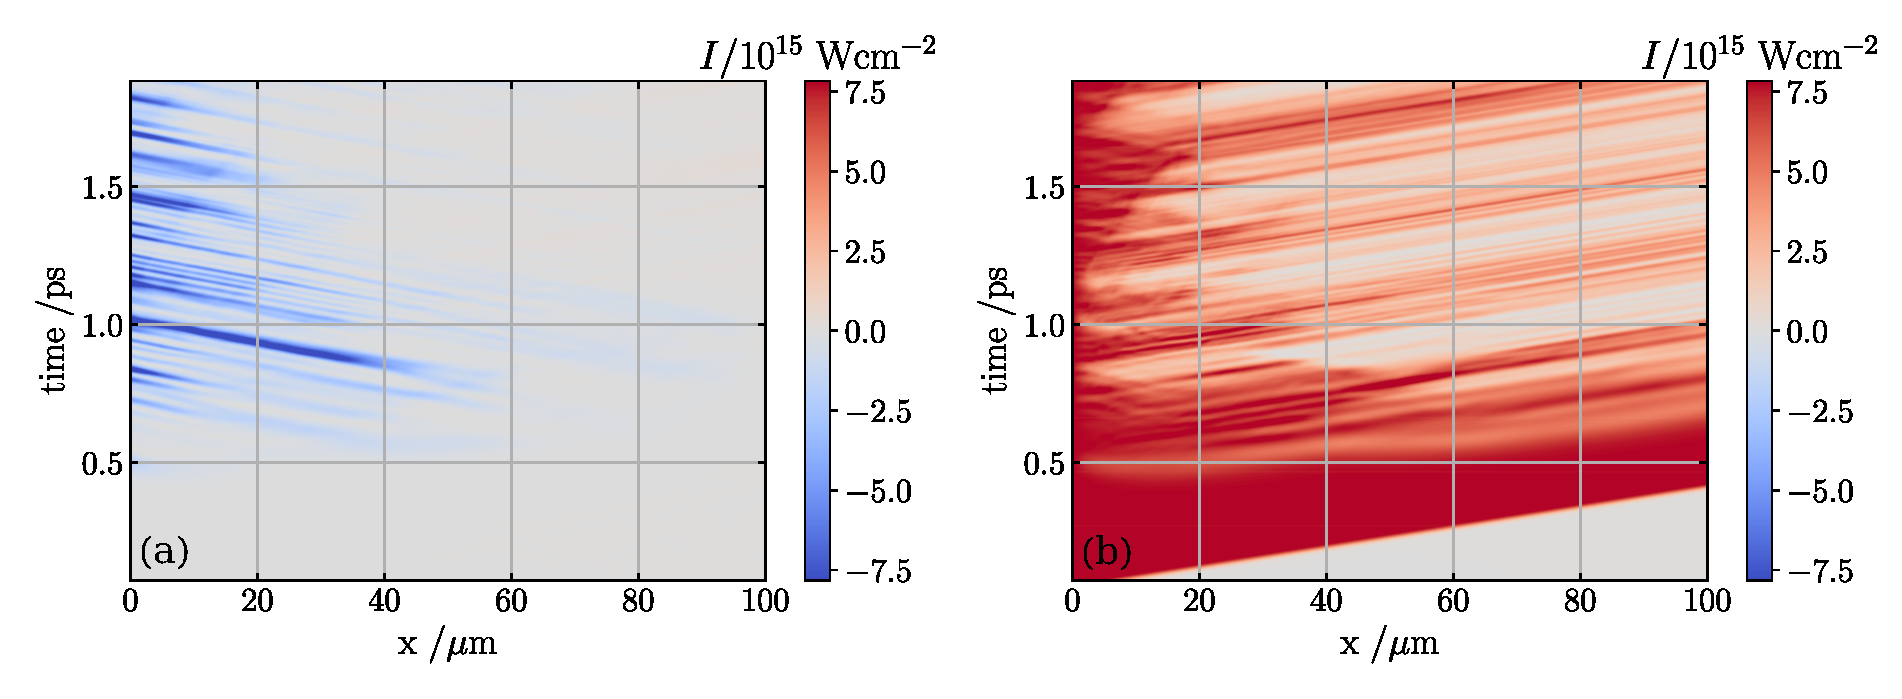
\includegraphics[width=\columnwidth]{Chapters/C4_iSRS/783e15_pump_depletion.pdf}
    \caption{(a) Poynting flux of scattered light (b) laser energy, showing significant depletion of the pump. Simulation parameters: $L_n = 500 \si{\micro\metre} $ centred at $0.15n_\mathrm{cr}$
    and $I_0 = 7.83\times10^{15} \si{W/\centi\metre^2}$. }
    \label{fig:pumpdepletion}
\end{figure}{}


Several saturation mechanisms for iSRS in PIC simulations have been proposed, depending on the physical mechanisms present in the simulation. For simulations in 1D with immobile ions, there are three possible saturation mechanisms for SRS undergoing autoresonance: wave-breaking of the plasma wave; pump depletion of the laser driver; and frequency shift such that the autoresonance condition is no longer satisfied. In simulations with mobile ions and in higher dimensions, additional saturation mechanisms have been identified for iSRS in a homogeneous plasma. These additional saturation mechanisms are: Langmuir decay instability (\acrshort{LDI}); wavefront bowing of the EPW; the trapped particle modulation instability (\acrshort{TPMI}); and self-focusing \citep{Yin2007}.

We can eliminate EPW wave-breaking as the saturation mechanisms in our simulations as the maximum normalised EPW energy well below the wave-breaking limit in all cases. Take, for example, the simylation corresponding to $I_0 = 7.83\times10^{15} \si{W/\centi\metre^2}$ on the red curve of Figure \ref{fig:paramScan} (a). We can calculate the wave-breaking limit across the density range to be $E_{\text{WB}} e/m_ec\omega_0 = 0.024 - 3.52 $; but the maximum EPW energy in the simulation is $E_{\text{EPW}} e/m_ec\omega_0 = 0.0056$, well below the limit.
Figure \ref{fig:pumpdepletion} shows the Poynting flux of the scattered light (a) and incident laser (b) for a simulation with intensity in the saturated regime ($I_0 = 7.83\times10^{15} \si{W/\centi\metre^2}$). We can see complete depletion of the pump correlated with the maximum intensity of scattered light first at approximately $x=45\si{\micro\metre}$, $t=0.8\si{\pico\second}$. It is interesting to note that iSRS at low densities is depleting the pump before it can reach higher densities, where the growth of SRS would be even greater. 

Finally, we consider saturation due to the non-linear frequency shift which destabilises the auto-resonance.


\section{Conclusion}\label{sec:conclusion}
Inflationary SRS has been detected in PIC simulations of a inhomogeneous plasmas
with parameters relevant to the shock-ignition model of ICF.
This study demonstrates an iSRS threshold
 $I_\mathrm{threshold} \lesssim 5\times 10^{15} \si{W/\centi\metre^2}$ across the whole range of parameters tested
 and that the location of this threshold depends on the density scale-length $L_n$. For the case with
$L_n=500 \si{\micro\metre}$ and $I_0 =4.83\times10^{15} \si{W/\centi\metre^2}$ significant iSRS  would occur
at $0.15 n_{\mathrm{cr}}$ generating hot-electrons with mostly $< 100 \si{\kilo \electronvolt}$ energies and
depleting the laser drive available at higher densities. This is potentially beneficial to
shock-ignition in that these electrons are likely to enhance the ignitor shock and prevent significant SRS at higher densities,
potentially absolute at $0.25 n_\mathrm{cr}$. SRS at higher densities is likely to
generate electron distributions with a higher percentage of
$> 100 \si{\kilo \electronvolt}$ electrons than that from iSRS at lower densities.
These results suggest that a potential route to use iSRS to the advantage of shock-ignition,
assuming all SRS cannot be removed by other means,
would be for the shock ignitor pulse to have the largest possible amplitude. This would ensure significant iSRS at lower
densities and generate only hot-electrons with energies below $100 \si{\kilo \electronvolt}$. This in turn would pump deplete the laser
reducing SRS at higher densities which could generate hot-electrons with energy above  $100 \si{\kilo \electronvolt}$. These conclusions are however only valid for the restricted 1D, collisionless simulations
presented in this paper and more detailed simulations, as outlined below, would be needed to fully assess the hot-electron
distribution and its impact on SI schemes.

The simulations presented in this paper highlight the importance of a thorough investigation of iSRS for any shock-ignition
plans. These results are however a first study of the plasmas parameters where iSRS may occur. A full theoretical
investigation of the potential impact of iSRS on shock-ignition will require significantly larger scale simulations. Of
particular importance are multi-dimensional effects and laser speckle profiles. These would allow the competition between
SRS and TPD as sources of hot-electrons to be assessed in two and three dimensions. The transverse non-uniformity associated with
multi-dimensional effects is likely to affect iSRS through trapped electron side losses and a broader spectrum of EPWs
resulting from side-scatter and TPD.
Furthermore, the auto-resonance responsible for iSRS in these simulations may not be
possible when a full speckle profile is included; since the extension of the resonance region may take the
resonant waves outside of an individual speckle. The use of broadband
laser systems to mitigate LPI will also need to be assessed
in the kinetic regime of iSRS.
All of these refinements to iSRS simulations will require considerably more
computing resources but are none-the-less needed for a comprehensive treatment of LPI relevant
to shock-ignition.

Talk more and cite about how things change as you move to higher dimensions

This work is nowhere near finished in fact it's a bit crap

Write a bit about Christoferetti's reviwers comments and how their must be some effect caused by the damping as well as autoresonance.

%\bibliography{Chapters/C4_iSRS/iSRS}


% !TeX root = ../../Thesis.tex
\chapter{Effects of laser bandwidth on inflationary stimulated Raman scattering}
\label{chp:broadbandSRS}

In this chapter, results of one-dimensional PIC simulations are presented, which represent the first investigation into the practical possibility of using broadband to suppress inflationary SRS in shock-ignition. The chapter begins with a review of the literature discussing suppression of SRS by broadband lasers. We then show that for a decoupled broadband laser, the non-linear frequency shift must be taken into account when calculating the condition for suppression of iSRS. Next we consider the case of realistic shock-ignition schemes on three laser systems: frequency-tripled Nd : glass; Krypton Fluoride (KrF); and Argon Fluoride (ArF). In each of these cases we model the predicted maximum realistic bandwidth in its physically-correct functional form. The chapter concludes with a discussion of the limitations of the modelling done so far, and suggestions for future work.

N.B. In this chapter, bandwidths are given in units of tera-Hertz (THz) since this is standard in the literature. This can be converted to radians per second through the relation $\Delta \omega = 2\pi \Delta f$. 

\section{Motivation and literature review}

Early results in the 1970s suggested that finite-bandwidth laser drivers could change the behaviour of parametric instabilities. These studies considered a variety of parametric instabilities, including: the parametric decay instability \citep{Thomson1974}; stimulated Brillouin scattering \citep{Kruer1973}; and stimulated Raman scattering \citep{raymer_theory_1979}. Recently, broadband suppression of parametric instabilities has, once again, become a fashionable topic of discussion. All lasers have some natural bandwidth, which arises from quantum effects. However, for the majority of lasers relevant to ICF, this natural bandwidth is far too small to affect parametric instabilities. There are various ways that additional bandwidth can be introduced into a laser system, including: induced spatial incoherence (\acrshort{ISI}) \citep{Lehmberg198327}; smoothing by spectral dispersion (\acrshort{SSD}) \citep{Skupsky1989}; stimulated rotational Raman scattering (SRRS).

As discussed in Chapter \ref{chp:iSRS}, Stimulated Raman Scattering (\acrshort{SRS}) is a parametric instability of major concern to shock ignition; since it scatters light away from the target, and drives electron plasma waves to large amplitudes which then damp and send hot electrons towards the cold fuel. As such, many people are interested in the possibility of using broadband laser systems to suppress the growth of SRS in shock-ignition coronal plasmas. In the following literature review, we consider each of the main forms of SRS separately: absolute; convective-fluid; inflationary; and multi-beam. The original work presented in this chapter focuses on inflationary SRS, but we believe that it must be place in its proper context by reviewing the literature for all types of SRS, since these are often concurrent and may all be present in the shock-ignition plasma corona.

\subsection{Absolute SRS}
\citet{Thomson1974} showed that for an absolute parametric instability, with homogeneous growth rate $\gamma_0$ driven by a laser with bandwidth $\Delta\omega$, if $\Delta\omega > \gamma_0$ then the growth rate of the instability is reduced by a factor of $\gamma_0/\Delta\omega$.

PIC modelling of absolute SRS at low density and temperature ($n_e=0.08n_{cr}$, $T_e=100\si{eV}$, corresponding to $\kld\sim 0.08$)
performed by \citet{Zhao2015} demonstrates the suppression of the SRS growth rate by frequency-modulated SSD-type bandwidth. They find that the suppression effect is increased by increasing the bandwidth; and that for a fixed bandwidth, the suppression depends on the modulation frequency. They also note that the bandwidth has no effect on the saturated level of SRS, only the growth rate. In their conclusion they stress the importance of considering the temporal structure of the laser field in each bandwidth investigation. In a follow-up paper \citet{Zhao2017July} consider SRS driven by incoherent light which is composed of a large number of beamlets each with different frequency and phase (called a decoupled broadband laser (DBL)).  For very large bandwidths (on the order of $10\%\omega_0$) they find that the growth rate of backward SRS is reduced compared to the frequency-modulated light with the same bandwidth, but that the scattered light still saturates at the same level as with no bandwidth.  

The work of \citet{Zhou2018} develops the theory of absolute-SRS suppression by \acrshort{DBL}-type bandwidth by considering the ``highly nonlinear", kinetic case where $\kld=0.3$. As well as confirming the suppression of the growth rate measured in \citep{Zhao2015,Zhao2017July}, they find that bandwidth in the range $2.25\%$ to $3.0\%$ actually acts to \emph{enhance} SRS in the so-called ``deep nonlinear stage" by increasing the resonant range in line with the non-linear frequency shift. The authors conclude that a broadband laser light is not an appropriate choice for suppression of absolute SRS on a several picosecond time-scale. 

\subsection{Fluid convective SRS}

We have seen, in the previous section, that absolute SRS can be suppressed using random bandwidth \citep{Thomson1974}; deterministic frequency-modulated bandwidth \citep{Zhao2015}; and bandwidth from a DBL \citep{Zhao2017July,Zhou2018}. This is not true, however, for convective SRS in an inhomogeneous plasma. It was shown by \citet{Guzdar1991} that bandwidth in the form of random phase modulation reduces the growth rate of SRS, but it also increases the length of the resonance region. For a system with the laser and plasma satisfying certain conditions, these two effects cancel out and the bandwidth has no net effect on the SRS gain. The conditions for exact cancellation are: the homogeneous growth rate and bandwidth are much smaller than the plasma frequency at the resonance point ($\gamma_0,\Delta\omega \ll \omega_{pe}(x_{\mathrm{res}})$); the length of the interaction region and coherence length are less than the plasma size $(\ell,c/\Delta\omega < L_x)$; and that the homogeneous growth rate is much smaller than the bandwidth $(\gamma_0 \ll \Delta\omega)$ \cite{Guzdar1991}. This analytical result tells us that random phase modulation will not be sufficient to suppress convective SRS.

It may be possible, however, to suppress convective SRS by using a decoupled broadband laser (\acrshort{DBL}). \citet{Zhao2017July} apply their theory of absolute SRS suppression in a homogeneous plasma by DBLs, to the case of convective SRS in an inhomogeneous plasma. For a plasma with a linear density profile and constant temperature such that $\kld \ll 0.25$ throughout, they compare the electrostatic energy present in the simulation in the cases $\Delta\omega_0=0, \Delta\omega_0=15\%$. They find that for the $15\%$ bandwidth case, the electrostatic energy is reduced compared to with zero bandwidth and conclude that the linear convective SRS has been suppressed \citep{Zhao2017July}. In a second paper the same year, \citet{Zhao2017October} consider the case of an inhomogeneous plasma density profile relevant to indirect-drive ICF. 

An analytic description of this effect is given in \citet{Zhao2019}; they find that SRS can be well-controlled for a laser beam structure of multiple frequency components and total bandwidth of a few
percent. By considering the frequency difference between any two beamlets, they find that
there is a critical frequency difference below which the SRS instability regions
for the beamlets overlap to form a single instability region. In this case, the
two beamlets can be coupled with one EPW, leading to a higher growth rate for
SRS. This effect is demonstracted in 1D PIC simulations, which show that SRS can grow to a high level if the beamlets satisfy this coupling condition, even if the total bandwidth is very large.

They derive a gain exponent for standard convective SRS driven by two
beamlets of different frequencies, and find that two beamlets are independent
when
\begin{equation}\label{DLB_threshold_inhomo}
\delta \omega_{0} \geq \frac{\pi n_{0} c\left(\omega_{0}^{2}-\omega_{p
e}^{2}\right)^{3 / 2}}{8 L \omega_{0} \omega_{L}^{2} \nu_{p}^{2}}.
\end{equation}
Importantly, this condition is independent of the amplitude of the incident
laser. In theory, this condition would allow us to construct a DBL to suppress
SRS in a large-scale inhomogeneous plasma, however, secondary amplification of
back-scattered light by one of the beamlets is a possibility. We must therefore
consider another threshold for this secondary amplification: $\delta\omega_0 >
\omega_{L1}-\omega_{L2}$ where $[\omega_{L1},\omega_{L2}]$ is the range of EPW
frequencies excited by SRS in the plasma (not including nonlinear frequency
shift).



The parameters considered in this study are
$\lambda_0=0.33\si{\micro\metre}$,
$T_e=2\si{\kilo\electronvolt}$, $n_e = [0.08,0.12]n_c$, giving $\kld \sim
[0.26,0.35]$, well within the kinetic regime for SRS.

\subsection{Inflationary SRS}

\citet{Wen2021} derive a condition for the maximum gain of SRS driven by a sinusoidally frequency-modulated broadband laser, when the velocity of the resonance point is equal to the group velocity of the back-scattered light for as long as possible. By tuning the plasma parameters and/or laser parameters away from this condition, they can increase the threshold for kinetic SRS \citep{Wen2021}. The maximum gain criteria is given by the expression:

\begin{equation}\label{eqn:maxGainCondition}
 \Delta\omega\omega_m = \omega_{pe}c / 2L_n,
\end{equation} and is verified through PIC simulations in the kinetic and fluid regimes. The left-hand side of Eq. \ref{eqn:maxGainCondition} represents the maximum chirp ($|\partial_t\omega_0(x,t)|$) of the laser, and the right-hand side gives an expression for the spatial detuning due to density inhomogeneity. Several simplifying assumptions are made by the authors which allow them to derive this expression for the spatial detuning. Most importantly for our work, they omit the contribution of the non-linear frequency shift in their calculation of the velocity of the resonance point. \todo{Estimate size of this contribution in my cases and hope it is ignorable}

A key result of this work is that the threshold for iSRS driven by a sinusoidally frequency-modulated laser is independent of the bandwidth or frequency modulation alone, rather it depends on their product. Figure \ref{fig:Wenreplication} shows results from our benchmarking of Wen's work. In this benchmarking study we recovered the results of their Osiris study using our own PIC code, EPOCH. We ran several simulations with fixed maximum normalised chirp ($\Delta\omega \omega_m / \omega_0=5.5\times10^{-6}$) and varied bandwidth. We find that the inflation threshold has a weak dependence on the bandwith alone. From this preliminary investigation, we were confident in our laser set-up and in the use of EPOCH for this project.


\begin{figure}[ht]
   \centering
    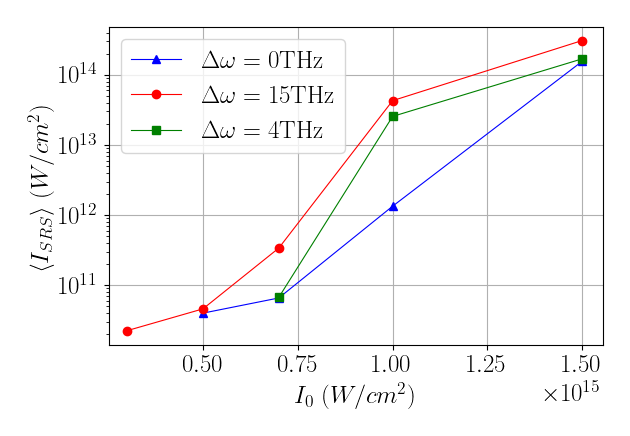
\includegraphics[width=0.75\columnwidth]{Chapters/C5_broadband/fig51_thesis.png}
    \caption{Intensity of light scattered by SRS, averaged over the last three picoseconds of each simulation, for three laser set-ups with fixed maximum normalised chirp ($\Delta\omega \omega_m / \omega_0=5.5\times10^{-6}$) and varied bandwidth. The simulation parameters common to all data-points are: $T_e = 4\si{\kilo eV}; L_n = 400\si{\micro\metre}; n_e(x) = 0.11n_{\text{cr}}\text{exp}(x/L_n);\text{PPC=16,000}. $}
    \label{fig:Wenreplication}
\end{figure}{}


\subsection{Multi-beam SRS}
Studies have also been performed using the code LPSE which show that, at ignition scales, absolute multi-beam backward SRS can be mitigated with bandwidth $\sim 1.6\%$ \citep{Follett2021}.

\section{Decoupled broadband lasers}

The work in this section was presented at the 62nd annual meeting of the American Physical Society Division of Plasma Physics in November 2020.
 
To begin our investigation of the effect of broadband on inflationary SRS, we focussed on the most relevant papers in the literature at the time (\citep{Zhao2019}) This body of work concerns convective SRS in an inhomogeneous plasma, driven by a decoupled broadband laser.


A decoupled broadband laser is defined in Ref \cite{Zhao2017July} as

\begin{equation}\label{eqn:DBL}
  a_{\mathrm{DBL}} = \sum_{i=1}^{N} a_i \mathrm{cos}(\omega_it + \phi_i),
\end{equation}
where $a_i,\omega_i,\phi_i$ are the amplitude, carrier frequency, and phase of
each of the $N$ beamlets. The central frequency and wavelength of the laser is
$(\omega_0,k_0)$ and the total frequency spectrum bandwidth is
$\Delta\omega_0$.

In \cite{Zhao2019} they consider the suppression of parametric
instabilities in a homogeneous plasma by decoupled broadband lasers
(\acrshort{DBL}). 

\subsection{Conclusions}
In conclusion, we decided not to pursue out investigation of DBL-type bandwidth any futher since a) there are no plans to impliment it on lasers of interest and b) 


\section{Realistic laser bandwidth}\label{sec:params}

This section concerns the results of our investigation into broadband suppression of inflationary SRS on different broadband laser systems. The particular form of the broadband may not seem like an important factor to us, but to the EPWs it can be very important.
We consider shock-ignition driven by three different laser systems: frequency-tripled Nd : glass lasers, such as the NIF and LMJ; KrF lasers; and ArF lasers. Each laser has a different frequency and native bandwidth. 

NRL provided us with density, temperatyre and intensity lineouts in 1D from simulations of shock-ignition on these these three laser systems. We selected a single time slice, just before the interaction pulse enters the under-dense plasma created by the assembly pulse. Their simulations were performed using the rad-hydro code \todo{Email and ask what code they used}

\begin{figure}[ht]
   \centering
    \includegraphics[width=\columnwidth]{Chapters/C5_broadband/a_b_c_d_Dens_temp.pdf}
    \caption{Sub-figures a), b), c) show density and temperature line-outs from NRL simulations at the end of the assembly pulse and the start of the ignition pulse. The laser is incident from the right, and the left-hand side boundary represents the quarter critical density surface. The green highlighted areas show the density and temperature range such that $0.3<\kld<0.45$. Sub-figure d) shows the final density and temperature profiles used for our campaign, defined by third order polynomials on the interval $[0,270\si{\micro\metre}]$, and with the laser incident from the left.}
    \label{fig:dens_temp}
\end{figure}{}


For all the simulations presented in this section, the following EPOCH parameters are constant: $\Delta x = \mathrm{min}_x(\lambda_D)$; $\mathrm{PPC} = 2000$; $T_{\mathrm{end}}=6\si{ps}$; thermal boundaries for particles; field boundaries are laser ($x_{\mathrm{min}}$), and absorbing boundaries ($x_{\mathrm{max}}$). We treat the ions as a neutralising background population to allow us to pinpoint the effect of bandwidth on inflationary SRS only. The incident laser intensity is set to be approximately the threshold intensity for inflationary SRS. The threshold intensity is found by varying the intensity for identical PIC set-ups to find the minimum intensity such that the time-averaged intensity of scatter from bSRS is greater than $10\%$ of the incident laser intensity. 

\renewcommand{\arraystretch}{1.25}

\begin{table}[h]\label{tab:laser}
\begin{center}
\begin{tabular}{|l|l|l|l|l|}
\hline
\begin{tabular}[c]{@{}l@{}}Wavelength /\\ nm\end{tabular} & \begin{tabular}[c]{@{}l@{}}Frequency \\ / THz\end{tabular} & \begin{tabular}[c]{@{}l@{}}Intensity / \\ $10^{15}\text{Wcm}^{-2}$\end{tabular} & \begin{tabular}[c]{@{}l@{}}Bandwidth / \\ THz\end{tabular} & \begin{tabular}[c]{@{}l@{}}Bandwidth / \\ $\%$ $\omega_0$\end{tabular} \\ \hline 

351   &  854 &  0.4 to 4.0  &  0, 1, 10 &  0, 0.12, 1.2 \\ \hline

248   & 1209 &   & 0, 3, 6  &  0, 0.25, 0.50   \\ \hline

193   & 1553 & $4\times 10^{15}$   & 0, 5, 8, 10  & 0, 0.32, 0.52, 0.64  \\ \hline
\end{tabular}
\end{center}
\caption{Laser parameters for this investigation. Where multiple values are presented in a list, each represents a different simulation. The incident laser intensity is set to be approximately the threshold intensity for inflationary SRS. The choice of bandwidths and their implementations in EPOCH are explained and referenced in Sections \ref{sec:351}, \ref{sec:248}, \ref{sec:193}, for the 351, 248, 193 nm cases respectively.}
\end{table}


\renewcommand{\arraystretch}{1.25}
\begin{table}[h]
\begin{center}
\begin{tabular}{|l|l|l|l|l|l|}
\hline
Wavelength / nm & $L_x$ /$\si{\micro\metre}$ & $T_e$ / keV & $n_e$ / $n_{cr}$ & $\omega_{pe}$ / $\omega_0$ & $L_n$ / $\si{\micro\metre}$
\\ \hline 
351 & 270 & 5.4 & $[0.105,0.175]$ & $[0.33,0.42]$ & $[420,590]$ \\ \hline
248 & 270 & 3.4 & $[0.078,0.137]$ & $[0.27,0.38]$ & $[400,550]$ \\ \hline
193 & 275 & 3.5 & $[0.071,0.140]$ & $[0.26,0.37]$ & $[330,470]$ \\ \hline
\end{tabular}
\end{center}
\caption{Table shows plasma parameters from simulations performed at the NRL, chosen such that $\kld$ is between 0.3 and 0.45. The temperature given is the maximum temperature of the particles initialised at $t=0$, as there is, in reality, a slight temperature gradient in the electron profile.}
\label{tab:plasma}
\end{table}

\renewcommand{\arraystretch}{1.25}
\begin{table}[h]
\begin{center}
\begin{tabular}{|l|l|l|l|l|l|}
\hline
$\lambda_0$ / nm & $n_e$ or $T_e$ & $a_0$ & $a_1$ & $a_2$ & $a_3$
\\ \hline 
351 & density & $1.05 \times 10^{-1}$  & $1.81 \times 10^2$ & $2.02 \times 10^5$ & $6.47 \times 10^8$ \\ \hline
351 & temperature & $5.28$ & $3.16 \times 10^2$ & $6.60 \times 10^5$ & $1.80\times 10^8$ \\ \hline
248 & density & $8.21 \times 10^{-2}$ & $1.52 \times 10^2$ & $2.46 \times 10^5$ & $3.55\times 10^8$  \\ \hline
248 & temperature & $3.58$ & $9.50 \times 10^2$ & $1.42\times 10^6$ & $-1.27 \times 10^9$ \\ \hline
 193 & density & $7.06\times 10^{-2}$ & $1.66\times 10^2$ & $3.95\times 10^4$ & $1.01\times 10^9$\\ \hline
 193 & temperature & $3.01$ & $1.47 \times 10^3$ & $1.31\times 10^6$ & $-2.27\times 10^9$ \\ \hline
\end{tabular}
\end{center}
\caption{Just trying to put in the coefficients somehow (193: $x_{max}$ = 272 microns) (248: $x_{max}$ = 271microns)}
\label{tab:coeffs}
\end{table}

\section{351nm Nd : glass laser}\label{sec:351}

\begin{figure}[ht]
   \centering
    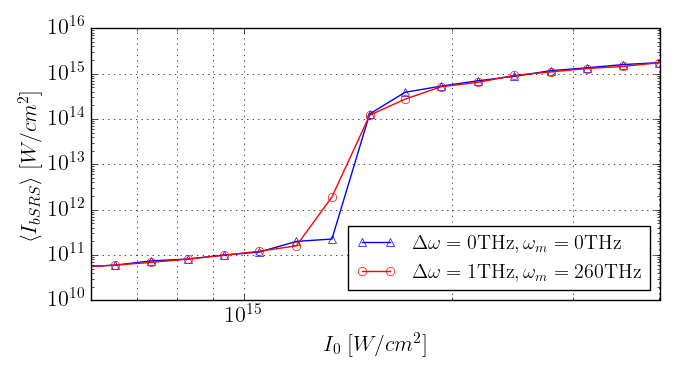
\includegraphics[width=\columnwidth]{Chapters/C5_broadband/351nm_delw1_delw0.png}
    \caption{Intensity of light scattered by backward SRS, time-averaged for all $t>2\si{ps}$. The incident laser intensity varies between $4\times10^{14}\si{W/cm^2}$ and $4\times10^{15}\si{W/cm^2}$.}
    \label{fig:351nm_base_threshold}
\end{figure}{}


\subsection{Base case: $\Delta f=0$}
As stated in Section \ref{sec:params}, the plasma density and temperature profiles are taken from the library of radiation hydrodynamic simulations at the Naval Research Laboratory. 

Sorry this is a horrible way to write this, but this is the detailed plasma set-up: $T_e(x) = \sum^3_{i=0} T_i x^i$, $n_e(x) = n_{\mathrm{cr}}\sum^3_{i=0} n_i x^i $;
$\{T\}_i  = \{3.01, 1.47\times10^3,1.31\times10^6,-2.27\times10^9\}$;
$\{n\}_i  = \{0.07, 165, 3.95\times10^4, 1.01\times10^9\}$. 



\subsection{SSD-type bandwidth: $\Delta f=1\si{THz}$}
1THz is the maximum bandwidth currently implemented by SSD on a 351nm laser, achieved at the Omega laser facility \citep{Regan2005}. According to \citet{Wen2021}, in order to increase the iSRS threshold we require that the modulation frequency satisfies $\omega_m \gg \omega_{pe} c / 2L_n\Delta\omega$. From the plasma parameters given in Table \ref{tab:plasma} and bandwidth of 1THz, this requirement becomes: $\omega_m \gg 128  \si{THz}$. This is problematic, since the optimal modulation frequency for SSD-type smoothing is on the order of $10 \si{GHz} = 0.001 \si{THz}$ \citep{Regan2005,Kelly2013}.

We can implement a continuous-bandwidth frequency-modulated laser in EPOCH using the standard EPOCH laser-driver like so:

\begin{equation}
\begin{aligned}
   E(x,t) &= E_0\text{sin}\left(\omega_0 t - \phi(x,t)\right) \\
   \phi(x,t) &= \frac{1}{2}\frac{\Delta\omega}{\omega_m}\text{sin}\left(\omega_mt - \frac{\omega_m}{c}x\right).
\end{aligned}
\end{equation}

\subsection{Optical parametric amplification: $\Delta f=10\si{THz}$}
According to \citet{Lehmberg2020} ``Parametric amplification may allow bandwidths up to 10 THz from 351 nm glass systems...".


\begin{figure}[ht]
   \centering
    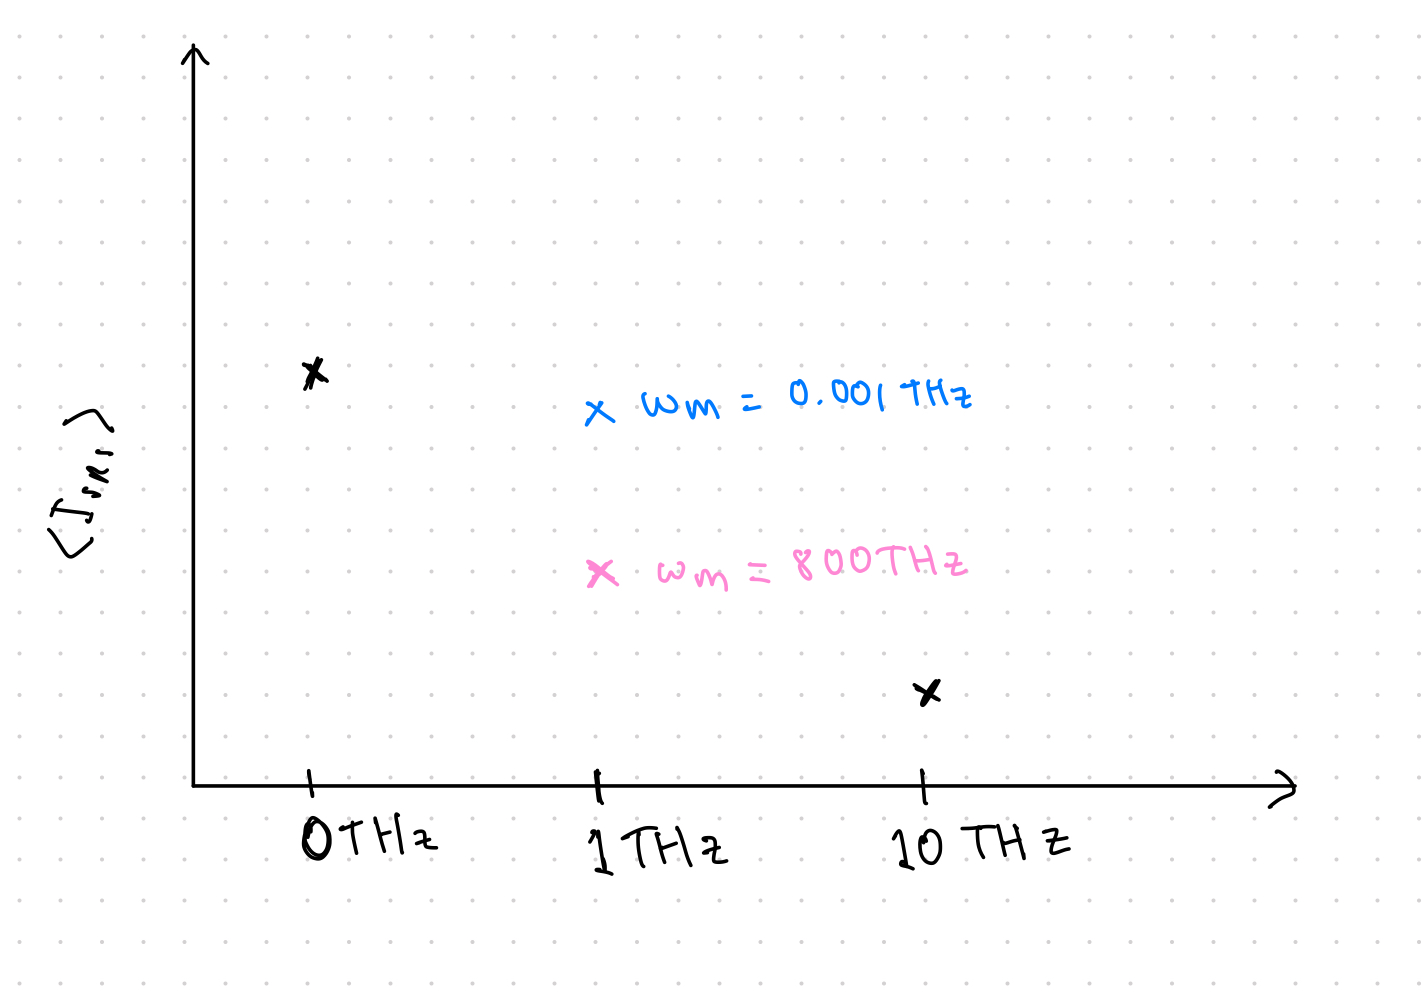
\includegraphics[width=0.75\columnwidth]{Chapters/C5_broadband/ndglass_placeholder.jpeg}
    \caption{placeholder figure for Nd glass sim results}
    \label{fig:NdGlass}
\end{figure}{}

\section{248nm krypton fluoride}\label{sec:248}

\subsection{Base case: $\Delta f=0$}




\subsection{Intrinsic bandwidth: $\Delta f=1,2,3$ $\si{THz}$}
Intrinsic bandwidth of KrF laser such as Nike is predicted to be 3Thz \citep{Obenschain15}

\subsection{Self phase modulation: $\Delta f=4,5,6$ $\si{THz}$}

According to this paper: "Stimulated rotational Raman scattering of arbitrarily polarized broadband light" \citep{Lehmberg2020} the SPM bandwidth of KrF limited to 6THz cos of physics.

\section{193nm argon fluoride}\label{sec:193}
Excimer lasers have a broad amplification spectrum in the UV when compared to Nd: glass lasers. In this section we consider the argon fluoride (ArF) laser under development at the NRL, which is predicted to have native bandwidth up to 10THz \citep{Obenschain2020}.

\subsection{Base case: $\Delta f=0$}



\subsection{Intrinsic bandwidth: $\Delta f =5,8,10$ $\si{THz}$}
In this section, we perform a series of simulations at different bandwidths which are considered realistic for ArF laser systems currently under development \citep{Obenschain2020}. To model the continuous laser spectrum, we follow the method presented in \citet{Bates2020} and distribute 50 beamlets of different frequencies around the central frequency. The intensities of the lines follow a Gaussian distribution whose FWHM is given by the laser bandwidth. \citet{Follett2019} says 50 is enough for a gaussian beam up to 10 percent. Each beamlet has a random phase so the total driven laser field looks like this:



\begin{equation}
\begin{aligned}
	E(x,t) &= \sum_{i=1}^{50} E_i \mathrm{sin}(\omega_i t + \phi_i) \\
	\phi_i & \in  [0,2\pi] \\
	\omega_i & \in [\omega_0 - \Delta\omega / 2, \omega_0 + \Delta\omega / 2]
\end{aligned}
\end{equation}

\begin{figure}[ht]
   \centering
    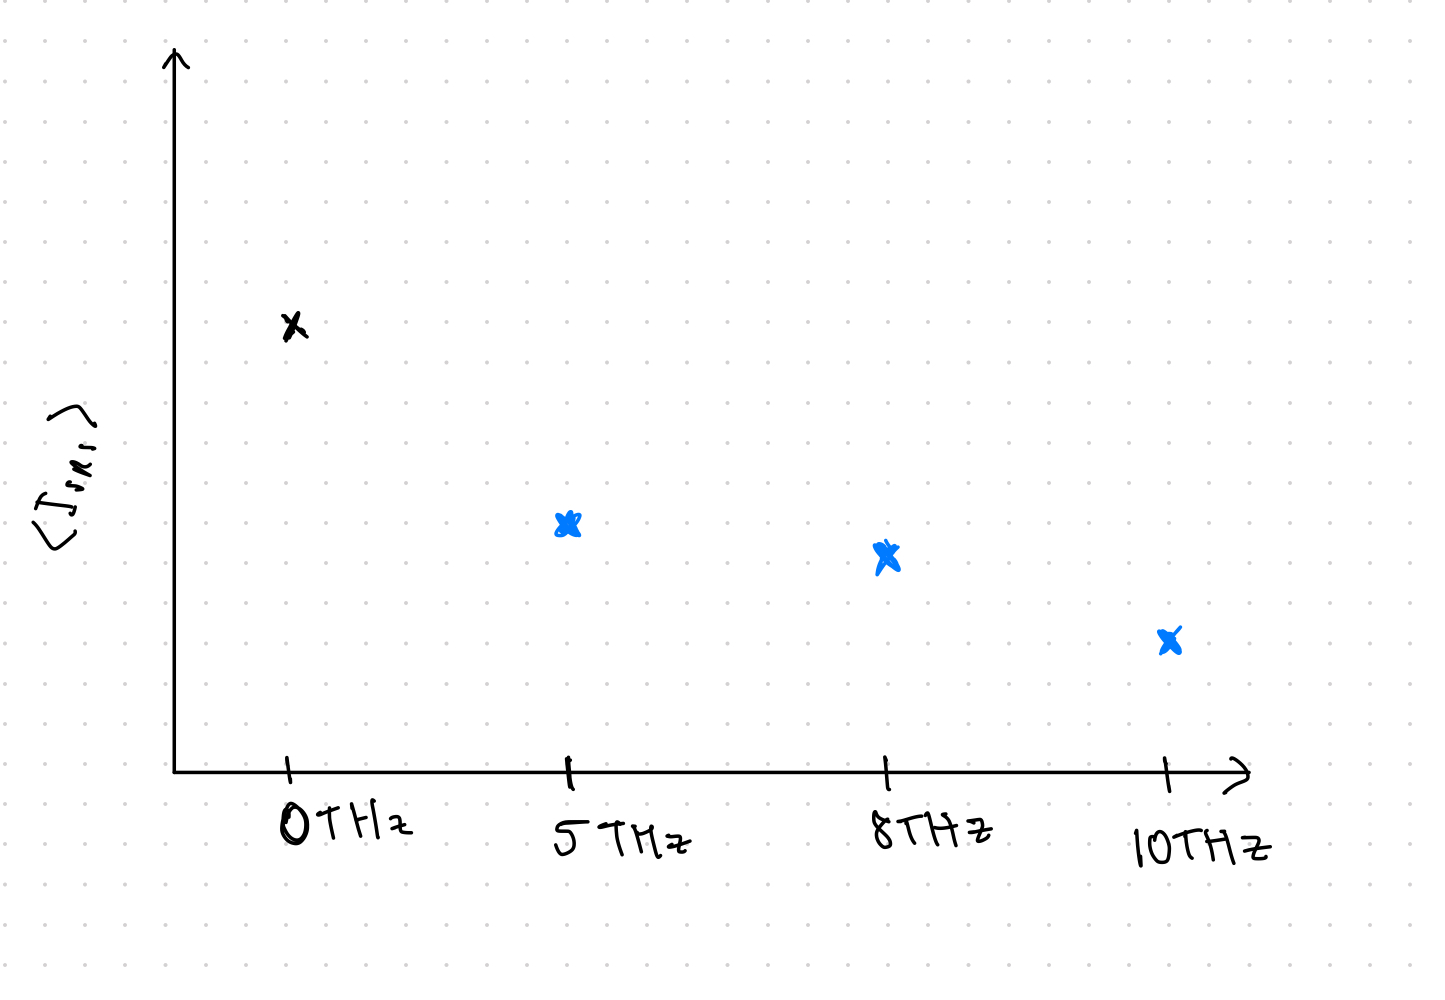
\includegraphics[width=0.75\columnwidth]{Chapters/C5_broadband/arf_placeholder.jpeg}
    \caption{placeholder figure for ArF sim results}
    \label{fig:ArF}
\end{figure}{}


\section{Conclusion}


%\bibliographystyle{plainnat}
%\bibliography{Chapters/C5_broadband/broadband}


% !TeX root = ../../Thesis.tex
\chapter{Effects of an External Magnetic Field on Stimulated Raman Scattering}
\label{chp:magSRS}

In this chapter, we present work performed while employed as a Junior Specialist at the University of California, San Diego between January and April 2020. The project was supervised by Professor Farhat Beg, and lead by Dr Adam Higginson (now at University of Boulder). The work presented (including data generated and data analysis) was carried out by the author, except in the cases outline below:
\begin{itemize}
\item Figure \ref{fig:SRS_LULI} was produced by M. Bailly-Grandvaux.
\end{itemize}

The chapter begins with a review of the literature which discusses the effect of an externally-applied magnetic field on stimulated Raman scattering. We then present modelling, performed by the author, of an experiment performed at the \acrlong{LULI} (France): J. R. Marqu\`es, P. Loiseau, J. B\'eard, A. Castan, B. Coleman, T. Gangolf, L. Lancia, A. Soloviev, O. Portugall, and J. Fuchs. Analysis of the SRS diagnostics was performed by J. R. Marq\`es, and (revisited) by M. Bailly-Grandvaux.  The experiment showed a small increase in SRS with an applied magnetic field, and this is recreated in our simulations. We then go on to investigate how the effect of the magnetic field depends on $\kld$ of the SRS electron plasma wave.

\section{Motivation and literature review}



Once again, wjhy is this a problem? why can we model in 1D? 

How can we continue to only consider modes without B field? Why no X or O modes?

GREAT PAPER it's fluid theory of SRS SBS competition in magnetised plasmas\citep{Vyas2016}

\subsection{Magnetic field suppresses kinetic SRS}

An electron plasma wave (\acrshort{EPW}) which propagates perpendicularly to a magnetic field experiences damping, caused by the trapped electrons being accelerated across the EPW wave-front and extracting energy from it. As was introduced in Chapter \ref{chp:theory}, inflationary stimulated Raman scattering (\acrshort{iSRS}), which takes place in a homogeneous plasma, depends on the damping of the EPW .

The first step of this research project was to replicate the results of \citet{Winjum2018}, in order to benchmark the EPOCH code against the results from OSIRIS and to understand the relevant diagnostics. 

here's a recent paper about 90T fields effect on SRS in inhomogeneous plasmas \citep{Zhou2021}. 



\begin{figure}[ht]
   \centering
    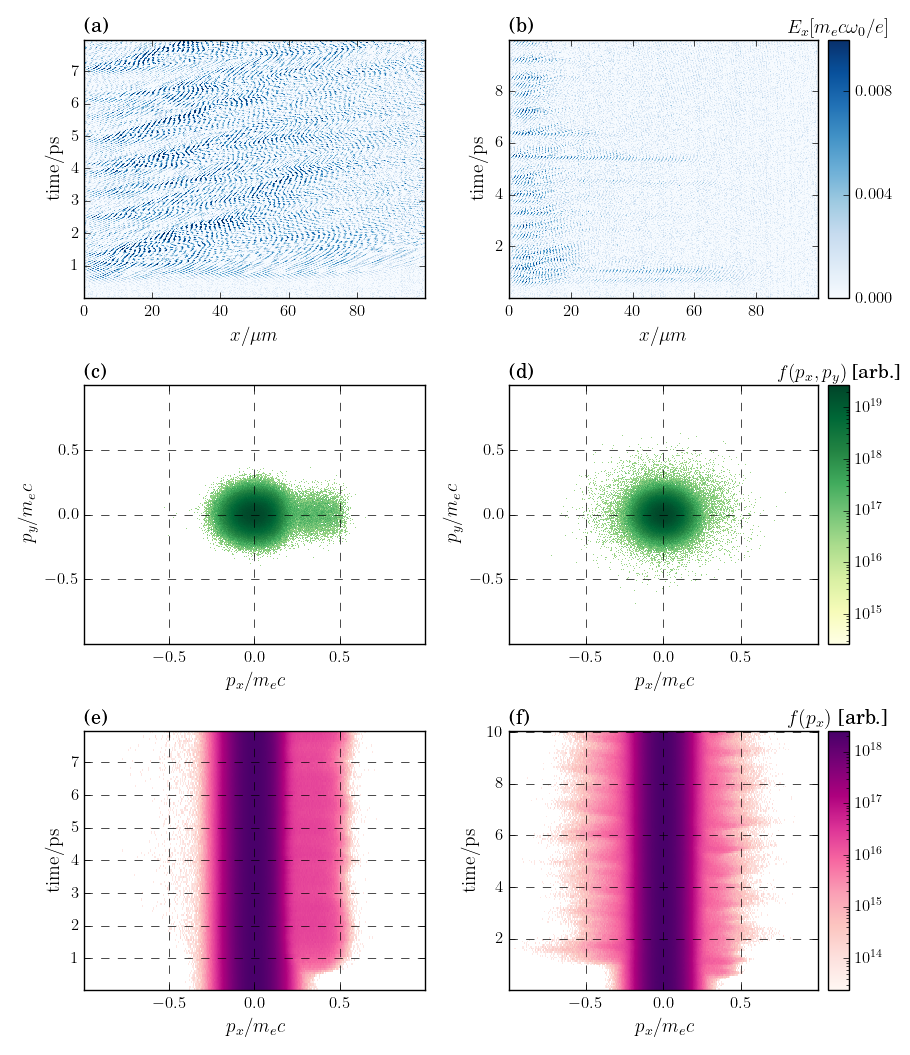
\includegraphics[width=\columnwidth]{Chapters/C6_magSRS/Winjum_rep_megaPlot.png}
    \caption{Electrostatic ($E_x$) field as a function of space and time. cf 0T (left) and 30T (right). Based on Figure 2 b. \citep{Winjum2018}}
    \label{fig:WinjumRep}
\end{figure}{}


Suppress SRS to reduce harmful electrons and reflectivity, or enhance if it actually makes good electrons (in the case of shock-ignition)

\subsection{Magnetic field could enhance kinetic SRS}

\subsection{What about fluid SRS?}

\section{Modelling SRS on LULI}
\subsection{Experimental results}
\begin{figure}[ht]
   \centering
    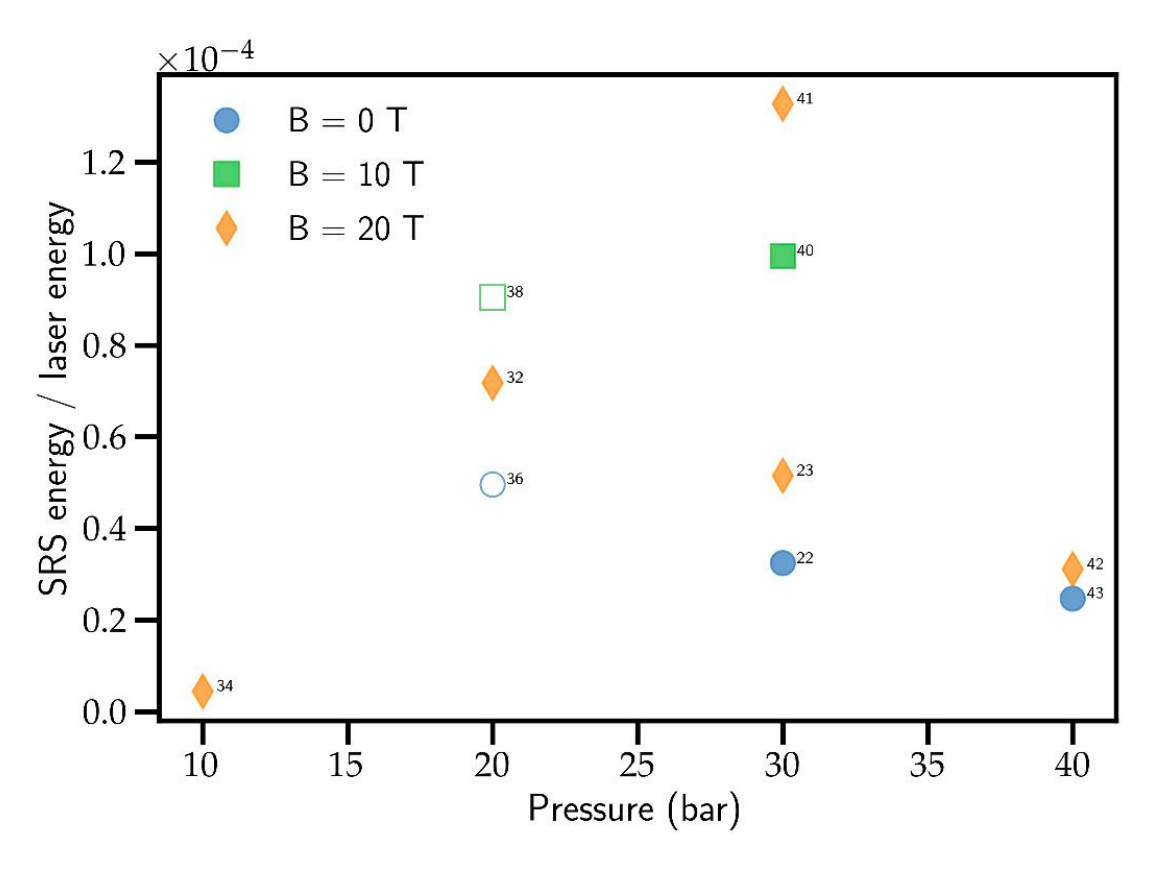
\includegraphics[width=0.8\columnwidth]{Chapters/C6_magSRS/SRS_LULI.png}
    \caption{\textbf{Figure produced by M. Bailly-Grandvaux.} Experimentally-measured SRS energy at different gas jet pressures, with and without magnetic fields. The solid-coloured markers represent shots with the laser  horizontally polarised with respect to the applied magnetic field, so that the laser magnetic field and applied magnetic field are parallel. The un-filled markers represent vertical polarisation of the laser.}
    \label{fig:SRS_LULI}
\end{figure}{}


\subsection{Simulation results}

Plasma density and temperature profiles at the centre of the gas jet were simulated using the FLASH code by Adam Higginson. 

\begin{table}[h]
\begin{center}

\begin{tabular}{|l|l|l|l|}
\hline
$n_e$ / $n_{\mathrm{cr}}$ & $T_e$ / eV & bSRS $\kld$ & fSRS $\kld$\\ \hline \hline
0.01 & 180 & 0.36 & 0.02 \\ \hline
0.025& 450 & 0.34 & 0.03 \\ \hline
0.05 & 600 & 0.27 & 0.04 \\ \hline
0.10 & 900 & 0.21 &  0.05\\ \hline
0.15 & 1100 & 0.18 & 0.06 \\ \hline

\end{tabular}

\end{center}
\caption{$T_i$ is $T_e/3$ in all cases}
\label{tab:LULI_setup}
\end{table}


\begin{figure}[ht]
   \centering
    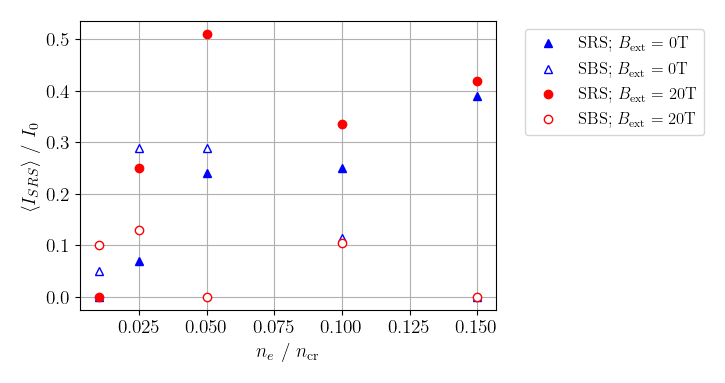
\includegraphics[width=\columnwidth]{Chapters/C6_magSRS/LULI_sims_v3.png}
    \caption{Reflected light from SRS and SBS (averaged over full simulation time) as a function of the initial homogeneous plasma density. Plasma densities and temperatures taken from FLASH simulations of single-beam shots without magnetic fields. The range of $\kld$ probed is 0.36, 0.34, 0.27, 0.21, 0.18.}
    \label{fig:LULI_sims_v3}
\end{figure}{}



\section{Magnetic field effect varies with plasma debye length}

\citep{Feng2018} REALLY good reference about SRS and LDI and anti-LDI

also don't forget this great paper about kld scling of iSRS autoresonance \citep{Chapman2013}

\subsection{Fixed ions: vary $\kld$}

Plasma parameters chosen to be relevant to LULI experiment (ish). $\lambda_0 = 1053 \si{\nano\metre}$; $L_x = 1000 \si{\micro\metre}$; $T_e = 1 \si{\kilo\electronvolt}$; $I_0 = 1\times 10^{15}\si{W/\cm^2}$; $T_{\mathrm{end}}=10 \si{ps}$; 1000 PPC (from convergence testing on $\left< I_{\mathrm{SRS}} \right>_{t>0}$).

\begin{table}[h]
\begin{center}

\begin{tabular}{|l|l|l|l|}
\hline
$n_e$ / $n_{\mathrm{cr}}$ & $\kld$ & regime & predicted behaviour\\ \hline \hline
0.02 & 0.55 & beyond ``loss of resonance" & no SRS, no dependence on $B_{\mathrm{ext}}$  \\ \hline
0.05 & 0.33 & strongly kinetic &  \\ \hline
0.08 & 0.25 & kinetic &  \\ \hline
0.11 & 0.20 & weakly kinetic & \\ \hline
0.20 & 0.12 & fluid & no dependence on $B_{\mathrm{ext}}$\\ \hline

\end{tabular}

\end{center}
\caption{Plasma density, $\kld$, regime, predicted behaviour}
\label{tab:predictions}
\end{table}

\begin{figure}[ht]
   \centering
    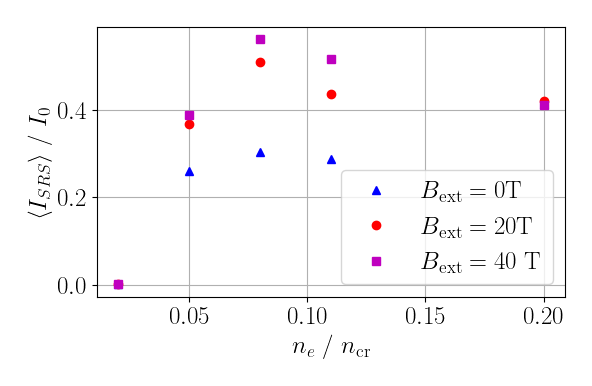
\includegraphics[width=0.9\columnwidth]{Chapters/C6_magSRS/kld_scan_SRS_scaling.png}
    \caption{Reflected light from SRS, averaged over the full simulation time, as a function of the initial homogeneous plasma density. By fixing the temperature at $T_e = 1\si{\kilo\electronvolt}$, the folowing values of $\kld$ are probed: 0.55, 0.33, 0.25, 0.20, 0.12. The following parameters are constant to all the simulations: 
 $\lambda_0 = 1056 \si{\nano\metre}$; $L_x = 1000 \si{\micro\metre}$; $T_e = 1 \si{\kilo\electronvolt}$; $I_0 = 1\times 10^{15}\si{W/\cm^2}$; $T_{\mathrm{end}}=10 \si{ps}$; 1000 PPC.}
    \label{fig:SRS_EPOCH}
\end{figure}{}


\section{Magnetic field effect changes with polarisation}






% !TeX root = ../../Thesis.tex

\chapter{Discussion}
\label{chp:discussion}


% !TeX root = ../../Thesis.tex
\chapter{Conclusions and Future Work}
\label{chp:conclusion}

\section{Conclusion}


\subsection{Does any of this matter?}

A recent paper by \citet{Nicholas2021} suggests that fusion energy (whether through ICF or magnetically confined fusion) will not be ready in time to act as a replacement for fossil fuels, which must be removed from the energy mix by the middle of the 21st century if we are to avoid the worst impacts of catastrophic climate change. They assume that, by the second half of the 21st century, renewable energies such as wind and solar will power most of the grid. However, the intermittent nature of these mechanisms will leave a gap in the energy market for a carbon-free source of baseload energy \citep{Nicholas2021}. In order for fusion energy to be a good choice for filling this gap it must be able to demonstrate its superiority over traditional nuclear fission power generation. This may include showing its better performance in terms of: waste production; ease of proliferation; and resource supply. In light of this analysis, the work presented in this thesis may never directly contribute to usable, or desirable, ICF energy-generation schemes.

\section{Future Work}
\label{sec:future-work}

\section{Summary}


%\appendix
%% !TEX root =  ../Thesis.tex

% !TEX root =  ../Thesis.tex

%\appendix{AIP Copyright contract}
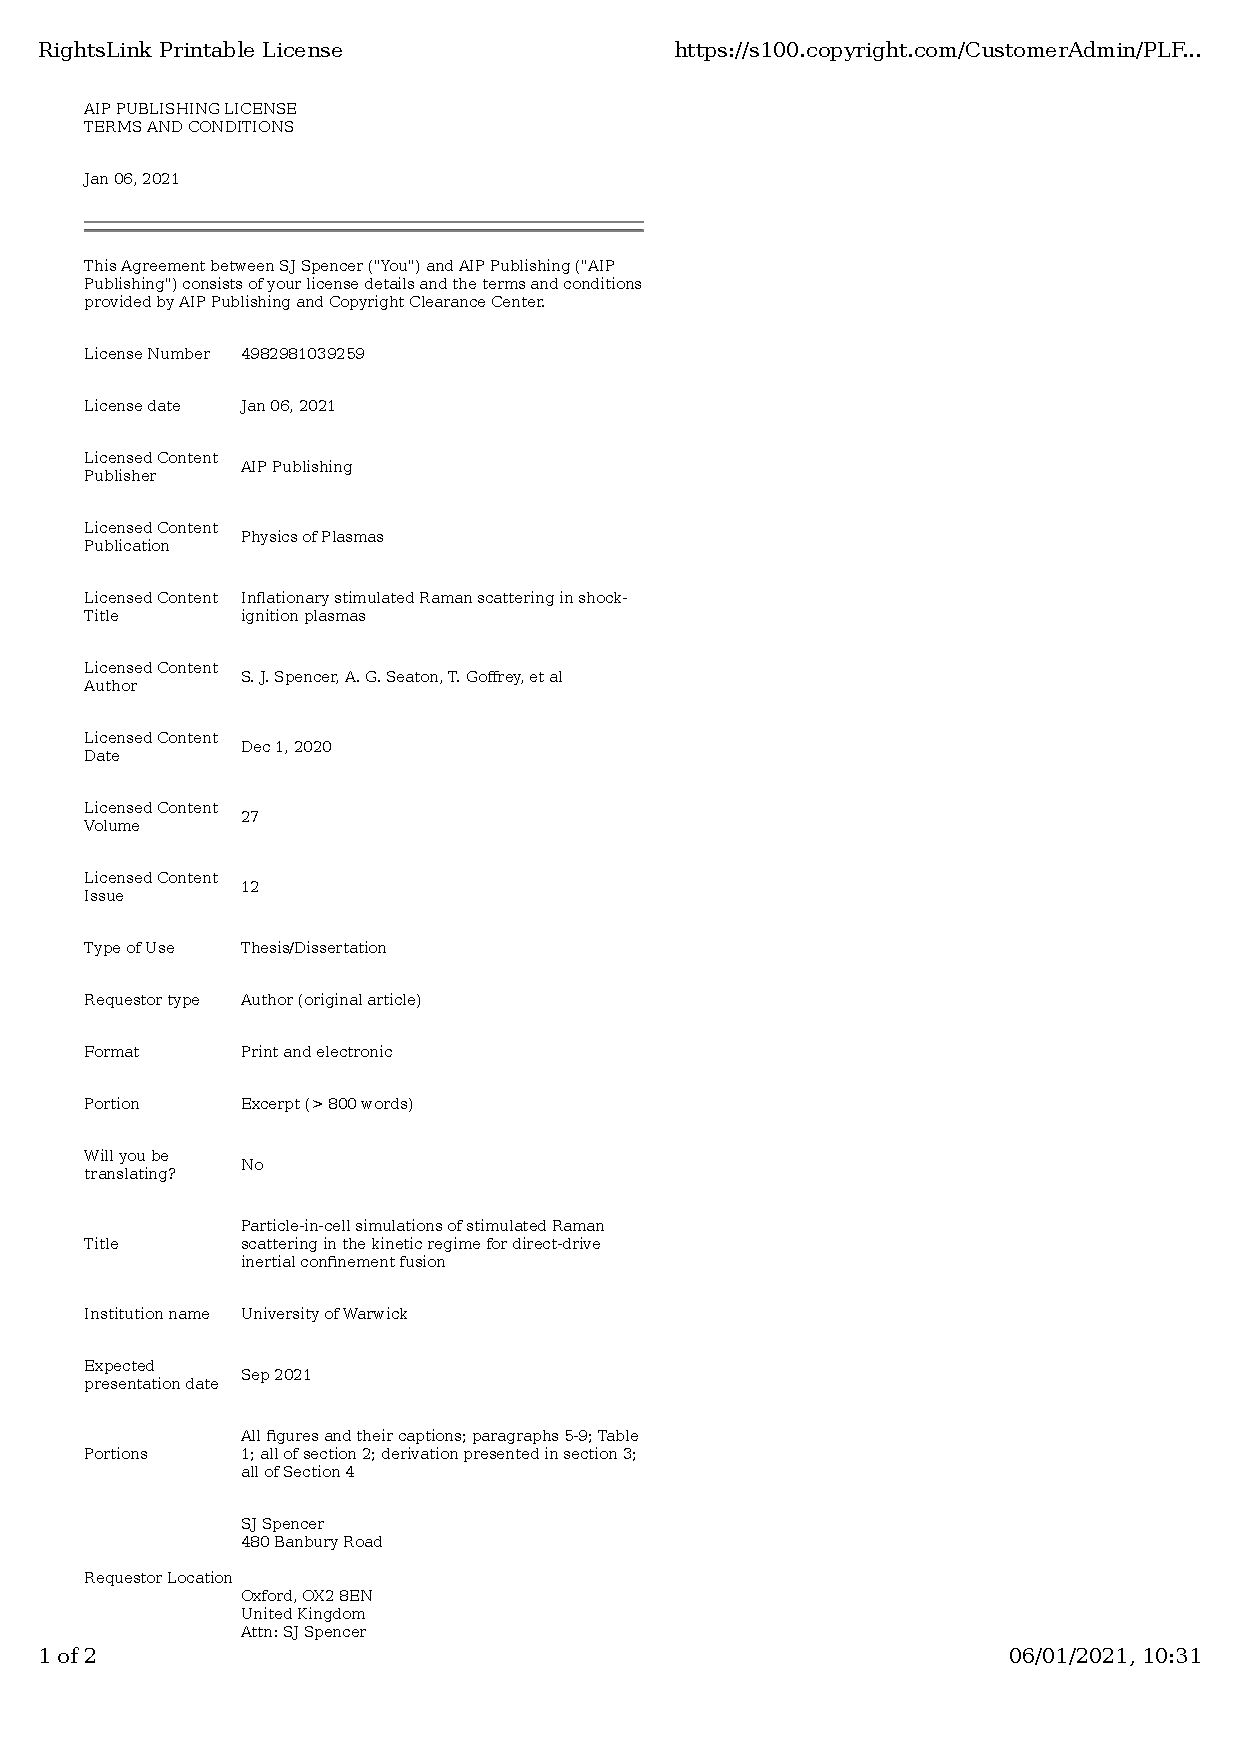
\includepdf[
	pages=-
]{Appendices/iSRS_license_agreement.pdf}


\renewcommand\bibfont{\small} % You might want a smaller bib font

\bibliographystyle{plainnat}
%\bibliography{Bib/bib}
%\bibliography{Chapters/C4_iSRS/iSRS}

\end{document}
